% 修士論文テンプレート

\documentclass[10pt]{jreport}

\usepackage{master_thesis}
\usepackage{./grad}
\usepackage[dvipdfmx]{graphicx}
\usepackage{here}
\usepackage{url}
\usepackage{bm}
\usepackage{comment}
\usepackage{cite}
\usepackage{amsmath,amssymb,amsfonts}
\usepackage{algorithmic}
\usepackage{graphicx}
\usepackage{textcomp}
\usepackage{xcolor}

% A4 : width 21cm, height 29.7cm
\usepackage[a4paper,textheight=21.7cm,top=3cm,left=2cm,right=2cm,headheight=15pt]{geometry}

\年度{2021}
\題目{VANETにおける車両位置とリンク状態を\\考慮した地理的opportunistic routing}
\指導教官{野口 拓, Alberto Gallegos Ramonet}
\学籍番号{6611200033-0}
\氏名{高橋 柊人}
\コース{計算機科学コース} %計算機科学コース or 人間情報科学コース


\begin{document}
% 表紙 %%%
\maketitle


\renewcommand{\thepage}{\roman{page}}
\setcounter{page}{1}
\addcontentsline{toc}{chapter}{内容梗概}
\chapter*{内容梗概}
本論文は, 筆者が立命館大学情報理工学研究科において行った「VANETにおける車両位置とリンク状態を考慮した地理的
opportunistic routing」の成果をまとめたものである.
近年, 通信インフラを用いることなく端末同士のみで通信を行うことができるアドホックネットワークを車両に応用した, 車両アドホックネットワーク(VANET)の研究が盛んにおこなわれている. VANETは緊急車両メッセージの伝搬, 事故情報の通知などにおける活用が期待されている. これらの用途を満たすために, VANETではルーチングが必要である. VANETのルーチングでは高速な移動性, ノードの不均一性, 建物による電波の妨害など様々な要件を考慮して設計する必要がある.
そこでVANET用のルーチングプロトコルとしてOpportunistic routingが注目を集めている.
Opportunistic routingではブロードキャストの性質を利用し, 受信したノード同士が協調しパケットを再ブロードキャストするか否かを決定することでパケット到達率の向上とオーバーヘッドの削減を果たしている. 
しかし, 多くの既存 Opportunistic routingは都市部を想定して設計されているにもかかわらず, 性能評価ではシミュレーションでシャドウイングの影響が考慮されていないため, 通信性能が過大評価されている可能性
がある. またそのことが原因でシャドウイングを考慮したルーチングプロトコルが設計されていない可能性がある. 
そこで, 本研究では, シャドウィングが既存ルーチングプロトコルに与える影響をネットワークシミュレータ
NS-3のシャドウイングモデルである Obstacle Shadowing Model を用いて調査し, シャドウイングが既存ルーチングプロトコルに与える影響を調査した. シミュレーションの結果, シャドウイングの影響を受けやすいシミュレーションシナリオでは, Geographic routingにおいて古くから知られているLocal optimum problemに陥る可能性が高まることを示した. 
これらの既存研究の問題点を解決するため, 本研究では新たにシャドウイングを考慮した交差点ベースのルーチングプロトコル (SIGO) を提案する. SIGO は中継ノードの優先度を決定するためのメトリックとして, 中継ノードと宛先ノードまでの距離, 中継ノードとの予想伝送確率に加えて, 交差点ノードであるかどうかを考慮する. シミュレーションにより,
パケット到達率の向上と, オーバーヘッドの削減を確認し, SIGO の通信性能の有効性を示した. 
また, Local optimum problemに陥った際には, Recovery Strategyと呼ばれる転送手法が必要である.
本研究では, 既存Recovery strategyは建物により電波が完全に遮断される前提を基にアルゴリズムが設計されているという問題点を解決するため, 新たなRecovery strategy(ORS)を提案する. 
シミュレーションの結果, ORSは既存Recovery strategyと比較してパケット到達率の向上と, オーバーヘッドの削減を確認し, ORSの通信性能の有効性を示した. 
最後に本研究で提案したSIGOをGeocast Routingに拡張し, Geocast routingにおいてもSIGOが有効な転送方式であることを示す. 


\newpage
\pagestyle{myheadings}
\renewcommand{\thepage}{\roman{page}}
%\setcounter{page}{1}
\addcontentsline{toc}{chapter}{目次}
%\setcounter{page}{1}
\tableofcontents


\newpage
\renewcommand{\thepage}{\arabic{page}}
\setcounter{page}{1}
\chapter{緒論}
\vspace{-5mm}

近年, 基地局を用いることなく端末同士のみで通信を行うことができるアドホックネットワークを車両に応用した, 車両アドホックネットワーク(VANET)の研究が盛んにおこなわれている. VANETは緊急車両メッセージの伝搬, 事故情報の通知などにおける活用が期待されている. これらの用途を満たすために, VANETではルーチングが必要である. VANETのルーチングでは高速な移動性, ノードの不均一性, 建物による電波の妨害など様々な要件を考慮して設計する必要がある. しかし, モバイルアドホックネットワーク(MANET)用に提案されている従来の方式\cite {3,4,5}ではVANETの複雑な要件を満たすことができない. そこで近年Opportunistic routing\cite{16}が注目を集めている. Opportunistic routingと従来のルーチングプロトコルとの主な違いは固定経路を使用せず, 送信ノードが次の中継ノードを1つに決定しないことである. Opportunistic routingではブロードキャストの性質を利用し, 受信したノード同士が協調しパケットを再ブロードキャストするか否かを決定することでパケット到達率の向上とオーバーヘッドの削減を果たしている. 

しかし, 既存Opportunistic routingの多くは都市部を想定して設計されているにもかかわらず, シミュレーション評価でシャドウイングの影響を考慮しておらず通信性能を過大評価している可能性がある. 実際, 802.11pチャネルでは建物による電波減衰が起こり, 道路沿いでは通信が制限されることが示されている\cite{17}. 

そこで本研究では, シャドウイングが既存ルーチングプロトコルに与える影響を明らかにし, 既存ルーチングプロトコルの問題点を考察する.
そして新たにシャドウイングを考慮したShadowing-based Intersection Geographic Opportunistic Routing(SIGO)と呼ばれるルーチングプロトコルを提案し, 都市環境での有効性を示す. 

本論文の構成は, \ref{Related}章ではVANETの説明とVANETにおける様々なルーチングプロトコルの特徴について述べる. \ref{LSGO}章では, VANET用に設計されたOpportunistic routingの代表的な手法の1つであるLSGOについて述べ, この手法の問題点について考察する. \ref{Proposed}章では, \ref{LSGO}章で紹介した問題点を解決するための提案手法について述べる. \ref{Evaluation}章では, 提案手法の性能評価について述べ, \ref{Conclusion}章で研究で得られた内容のまとめ, 今後の課題について述べる. 



\chapter{VANET}
\label{Related}
\vspace{-5mm}
\section{概要}
近年, 情報通信技術の発達により, 無線通信を用いて車両間または, 路車間で情報をやり取りすることによって交通事故や渋滞などの道路交通問題の解決を目指す高度道路交通システム(ITS: Inteligent Transport System)が注目を浴びている\cite{1}. ITSの代表的なサービスとして, 渋滞情報と連動した高度なナビゲーションシステム(VICS: Vehicle Information and Communication System)\cite{VICS}や, 自動料金収受システム(ETC: Electronic Toll Collection)\cite{ETC}などがあげられる. これらのサービスを支える技術として, 車車間通信と路車間通信を組み合わせた車両アドホックネットワーク(vehicular ad-hoc network: VANET)がある. 路車間通信は車両が路側機のインフラ設備との無線通信により情報のやりとりを行う. しかし, 路車間通信はインフラ設備の設置にかかる費用と, 設置場所が限定される可能性があるという問題が存在する. 一方, 車車間通信は車両同士で通信を行うためインフラ設備の整備されていない不特定の場所でも通信を行うことが可能になる. VANETのアプリケーションとして, 渋滞回避情報の伝搬, 緊急車両情報の警告など, 安全運転支援などに期待されている. 
\section{車車間通信}
車車間通信は車両と車両との間で無線通信を行い, 情報のやり取りを行うものである. 車車間通信を図2.1に示す. 車車間通信では, 端末同士(車両同士)で自律的にネットワークを構築し, 宛先に直接通信できない場合には間の車両が中継車両となり, マルチホップ通信を行う. 車車間通信のメリットは固定のインフラを必要とせず車両間のみで通信が可能になり, インフラが存在しない地点で通信が可能になることである. 

\section{路車間通信}
路車間通信は, 道路に設置された路側機(RSU: Road Side Unit)と車両で無線通信を行い 
様々な情報の交換を行うものである. 路車間通信を図\ref{fig:VANET}に示す.  路車間通信の代表的なサービスとしてVICS(Vehicle Information and Communication System)やETC(Electronic Toll Collection)がある. VICSは, 各道路に設置されたビーコンから道路交通情報を発信し, 車載のカーナビや高速道路の電子掲示板に高速道路の渋滞の情報, 区間を通過するための所要時間, 駐車場情報などを表示する「ナビゲーションシステム高度化」を目指したサービスである. ETCは高速道路の入り口に設置されている通信機と車載の通信機で無線通信を行い, 料金所に止まることなく, 自動でスムーズに料金の支払いができるシステムである. 料金所での一時停止が渋滞の原因の一つであったが, ETCの導入で渋滞を解消することができた. 




%図の入れ方
\begin{figure}[!ht]
\centering
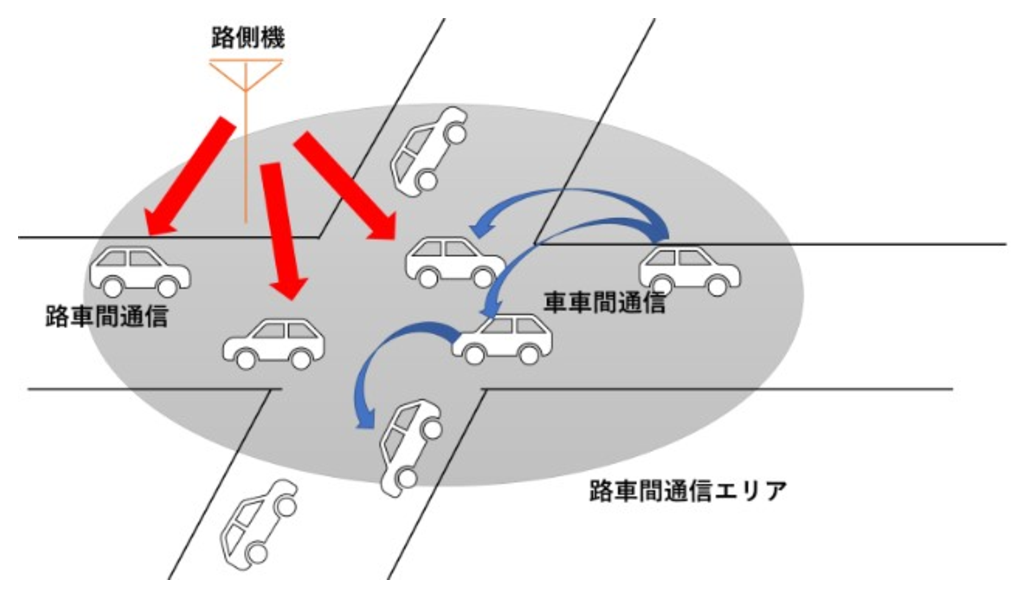
\includegraphics[width=15cm]{figures/VANET.eps}
\caption{車車間通信と路車間通信}
\label{fig:VANET}
\end{figure}


\section{ルーチングプロトコル}
\label{RoutingProtocol}
VANETを都市環境で展開する場合, 高速な移動性, 不均一な車両密度, 樹木や建物による電波の遮断など様々な要件を考慮する必要がある. この様々な要件に対応するため, 多種多様なルーチングプロトコルが提案されている\cite{2}. 次節以降でそれぞれのルーチングプロトコルの特徴について述べる.

\subsection{Topology-based routing}
\label{Topology}
Topology-base routing\cite {3,4,5} は, ネットワークに存在するリンクに関する情報を使用して, パケット転送を行う方式である. Topology-based routingはProactive型とReactive型に分類できる. 前者は, ノード間で周期的な制御パケットの交換を行うことにより, 各ノードがすべての宛先ノードへの経路情報を常時保持する方式である. 後者は, 最初は経路情報は保持しておらず, 通信要求が生じてから, 制御パケットを交換し経路情報を作成する方式である. 前者と比較して後者は, 制御パケットのオーバヘッドを抑えられるというメリットがある. 
しかし, これらのTopology-based routingは, ノードが頻繁に移動するVANETにおいては, 経路情報を定期的に更新する必要がある.
したがって, 制御パケットのオーバーヘッドが増加するためVANETには適していない.

\subsection{Geographic routing}
\label{Geographic}
Geographic routing\cite{6,7,8,9,10,11,12,13,14,15} は, 隣接ノードの位置情報と宛先ノードの位置に基づいてパケット転送を行う方式である. このタイプのルーチングプロトコルは, Topology-based routingのように確立されたルートを維持する必要がない. したがってGeographic routingは制御パケットを使用する必要がないため, 少ないパケット数でトポロジーの変化に対応することができる. Greedy fowardingはGeographic routingにおいて有名な方式の一つである. Greedy fowardingは隣接ノードの中で最も宛先ノードに近いノードを中継ノードとして選択することで, ホップ数やオーバヘッドの削減をしている. しかし, 実際の都市環境では, 建物によるシャドウイングや距離による電波強度の低下によりパケットのドロップ率が高くなる可能性がある. 

\subsection{Opportunistic routing}
\label{Opportunistic}
上記のルーチングの問題点を解決できる可能性がある, Opportunistic routing\cite{16} が近年注目を集めている. Opportunistic routingと前述したルーチングプロトコルとの主な違いは固定経路を使用せず, 送信ノードが次の中継ノードを1つに決定しないことである(図\ref{fig:Gegraphic_opportunistic}). Opportunistic routingではブロードキャストの性質を利用し, 受信したノード同士が協調しパケットを再ブロードキャストするか否かを決定することでパケット到達率の向上とオーバーヘッドの削減を果たしている. 

Opportunistic routingは主に次の4ステップで構成されている.

\begin{itemize}
	\item 中継候補ノードセット(RCS) の選択
	\item RCSの優先順位を決定
	\item RCSへのブロードキャスト
	\item 優先順位に応じた再ブロードキャストをするか否かの決定(RCS同士の協調)
\end{itemize}

図\ref{fig:Basic1}, \ref{fig:Basic2}にOpportunistic routingの基本モデルを示す.
$N_{s}$が送信ノード, $N_{d}$が宛先ノードである. 送信ノード$N_{s}$はRCSとして$N_{1}$ ~ $N_{n}$を選択する. 次に送信ノードは選択したRCSそれぞれに優先順位を指定してパケットをブロードキャストする. 受信した$N_{1}$ ~ $N_{n}$のノードはそれぞれ自身の優先順位を確認し, 中継タイマー(待ち時間)を設定する. 中継タイマーは優先順位が高いノードほど早くタイムアウトするように設定し, タイマーが切れたノードから再ブロードキャストを行う. 自身の中継タイマーが切れる前に自身より優先順位が高いノードの再ブロードキャストを受信した場合, 自身の再ブロードキャストをキャンセルし, 冗長なパケットの増加を防ぐ.
 

\begin{figure}[!ht]
	\centering
	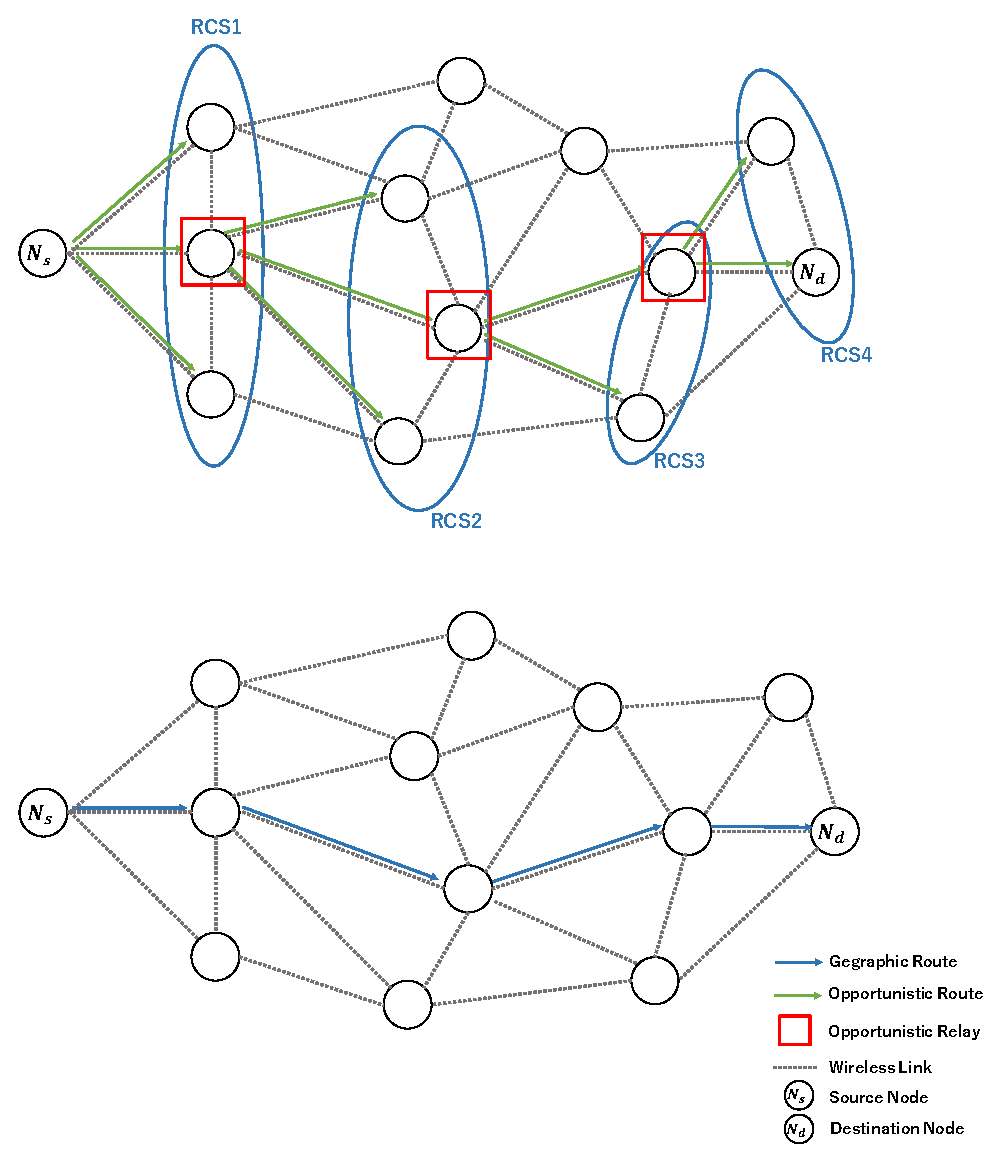
\includegraphics[width=150mm]{figures/difference_geographic_opportunistic.eps}
	\caption{Geographic routingとOpportunistic routing}
	\label{fig:Gegraphic_opportunistic}
\end{figure}

\begin{figure}[!ht]
	\centering
	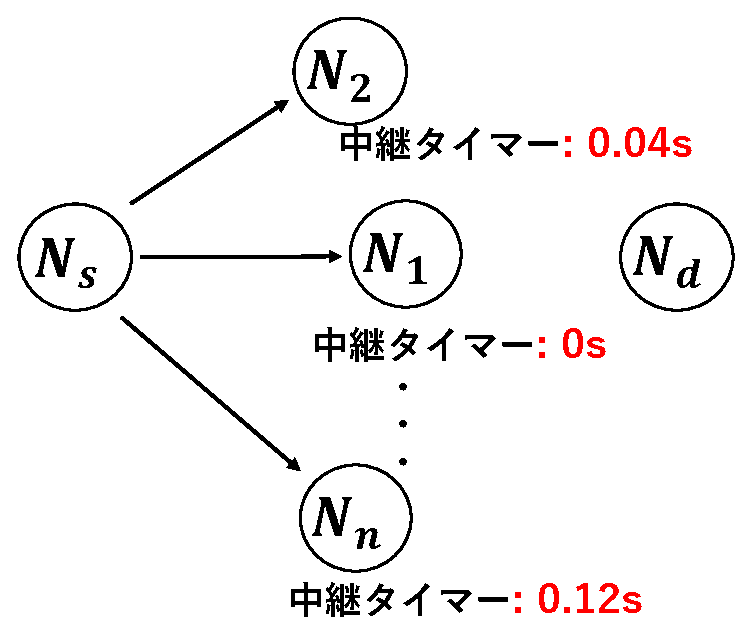
\includegraphics[width=90mm]{figures/basic-opportunity1.eps}
	\caption{Opportunistic routingの基本モデル1}
	\label{fig:Basic1}
\end{figure}

\begin{figure}[!ht]
	\centering
	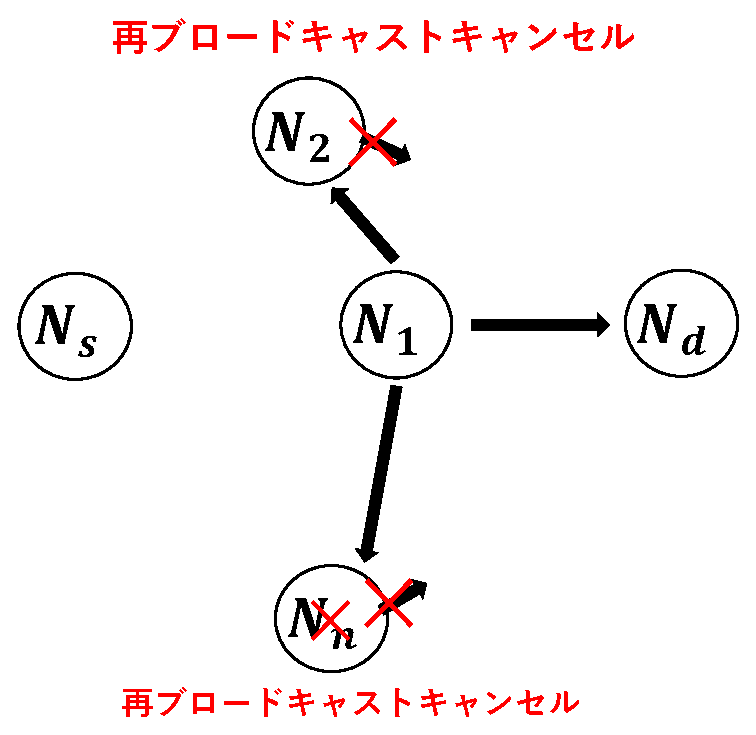
\includegraphics[width=90mm]{figures/basic-opportunity2.eps}
	\caption{Opportunistic routingの基本モデル2}
	\label{fig:Basic2}
\end{figure}

これらのことから, Opportunistic routingにおいて, 優先順位決定アルゴリズムが通信性能に直接影響を及ぼすことがわかる.

代表的なOpportunistic routingとしてOpportunistic multi-hop routing fo wireless networks (EXOR) \cite{16}が提案されている. これは, RCSの優先順位を決定するメトリックとして, Expected transmission cost (ETX) \cite{21}を用いている. しかし, ETX値はVANETの性質であるノードのランダムで高速なモビリティを考慮していないという問題がある.

そこで, 新たにVANETに適したETX値を考案したLink state aware geographic opportunistic routing protocol (LSGO) \cite{18}が提案された. LSGOでは, VANET用に最適化されたETX値をRCSの優先順位を決定するメトリックとして使用し, パケット到達率の向上, エンドツーエンド遅延の減少を実現している. また, Collision-aware opportunistic routing protocol (SCAOR) \cite{22}では, パケットの衝突でネットワークパフォーマンスを低下させる問題を防ぐために, ノード密度パラメータをRCSの優先順位を決定するメトリックとして追加した. その結果, 高速道路においてEXORやLSGOに比べ通信性能が向上することを示している. Hybrid opportunistic and position-based routing  protocol (OPBR) \cite{23}では, パケットがRCSに到達しない場合, 遅延が増加するという問題を解決するために, 隣接ノードの位置情報からリンクの切断を推測した. この結果パケット到達率の向上, エンドツーエンド遅延の減少を示している.

しかし, 既存のOpportunistic routingの多くは, 都市環境を想定して考案されているが, 性能評価で建物によるシャドウイングの影響が考慮されておらず, 通信性能を過大評価している可能性がある. また, これによりシャドウイングの影響を考慮したルーチングプロトコルが設計されていない可能性がある. 

そこで, 本研究では, 既存Opportunistic routingであるLSGOをネットワークシミュレータNs-3\cite{19}のシャドウイングモデルであるObstacle Shadowing Model\cite{20}を用いて評価し, 建物によるシャドウイングが起こる場合と起こらない場合の通信性能を検証し, 問題点を明らかにする.

\ref{Topology}, \ref{Geographic}, \ref{Opportunistic}節で紹介したプロトコルの特徴を表\ref{tab:protocol}に示す.

\begin{table}[h]
	\begin{center}
	\caption{ルーチングプロトコル比較}
	\label{tab:protocol}
	\centering
	\begin{tabular}{clllll}
		\hline
	    ルーチングタイプ & 制御パケット & パケットタイプ & 位置情報サービス & パケット到達率 & オーバーヘッド \\
		\hline \hline
		Topology & あり & ユニキャスト & なし  & △ & × \\
		Geographic  & なし & ユニキャスト & あり   & △ & 〇 \\
		Opportunistic & なし & ブロードキャスト & あり   & 〇 & △ \\
		\hline
	\end{tabular}
	\end{center}
\end{table}




\subsection{Geocast routing}
これまでの節では, ある特定ノードにデータを届けるUnicast routing protocolを紹介した.
本節では, ある特定領域にいる全ノードにデータを届けるGeocast routing protocol\cite{Geocast}について紹介する.
特定領域にいる多くのノードに情報を届けるために, 最も単純な方式がフラッディング手法である.
しかし, フラッディング手法はパケットを受信したすべてのノードがブロードキャストをするため, ブロードキャストストームの発生する確率が高まる.
そこで, 宛先方向へのフラッディングを行う指向性フラッディングがある. 指向性フラッディングの代表例として, Location-Based-Multicast (LBM) \cite{LBM}が提案されている.
LBMでは, 宛先領域(Geocast Region)と転送エリアを表す(Forwarding Region)を用いるLBM Scheme1, データパケットを受け取ったノードが, 自身と宛先領域の中心座標との距離を算出し, 自身が送信ノードより宛先領域の中心座標に近い場合のみデータパケットを転送するLBM Scheme2の2種類の転送手法が手案されている.
Scheme1, Scheme2の動作例を図\ref{fig:scheme1}, \ref{fig:scheme2}に示す.

\par
\vspace{5mm}
\noindent
\textbf{LBM Scheme1}
\vspace{5mm}

Scheme1の手順を以下の(1)~(4)に示す.


\textbf{手順 1} ソースノード$S$は, 矩形領域$OPQB$をGeocast regionとして指定する.

\textbf{手順 2} $S$は, 自身とGeocast regionを含む最小の矩形$ASCB$をForwarding Regionとして指定する. その後, Forwarding Regionの情報を含めたデータパケットをフラッディングする.

\textbf{手順 3} データパケットを受信したノードは,自身がForwarding Region内にいる場合,自身とGeocast Regionを含むForwarding Regionを再設定しフラッディングを行う.自身がForwarding Region外にいる場合,データパケットを破棄する.

\textbf{手順 4} Geocast Regionに到達するまで手順3を繰り返す. 


\begin{figure}[!ht]
	\centering
	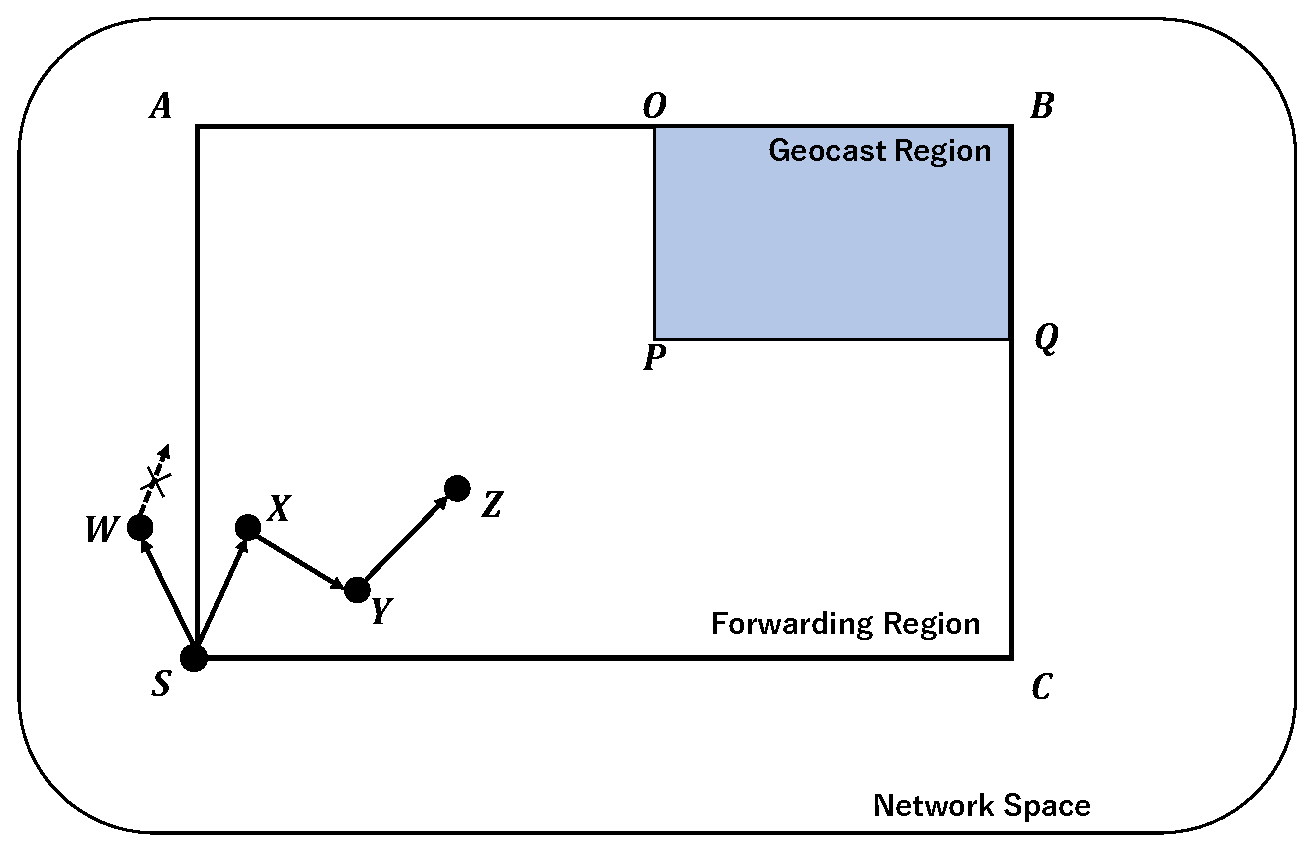
\includegraphics[width=100mm]{figures/Scheme1.eps}
	\caption{LBM: scheme1}
	\label{fig:scheme1}
\end{figure}

\par
\vspace{5mm}
\noindent
\textbf{LBM Scheme2}
\vspace{5mm}

Scheme2の手順を以下の(1)~(3)に示す.


\textbf{手順 1} ソースノード$S$は, Multicast Regionの中心座標と自身の位置情報を含めたデータパケットをフラッディングする.

\textbf{手順 2} データパケットを受信した各ノードは, 1ホップ前のノード(ノード$X$の場合のノード$S$)の位置情報と, 自身の位置情報を確認し, それぞれのMulticast regionの中心座標までの距離($Dist$)を算出する. 1ホップ前のノードより自身がMulticast regionの中心座標に近い場合, データパケットに自身の位置情報を再設定しフラッディングを行う.
例えば, 図の場合$Dist_x$ \verb|<| $Dist_s$の関係が成り立つため, ノード$X$はノード$S$からパケットを受信した場合, フラッディングを行う. しかし, $Dist_x$ \verb|<| $Dist_y$の関係が成り立つ, ノード$X$からのパケットをノード$Y$が受信した場合, データパケットを破棄する.

\textbf{手順 3} Geocast Regionに到達するまで手順2を繰り返す.



\begin{figure}[!ht]
	\centering
	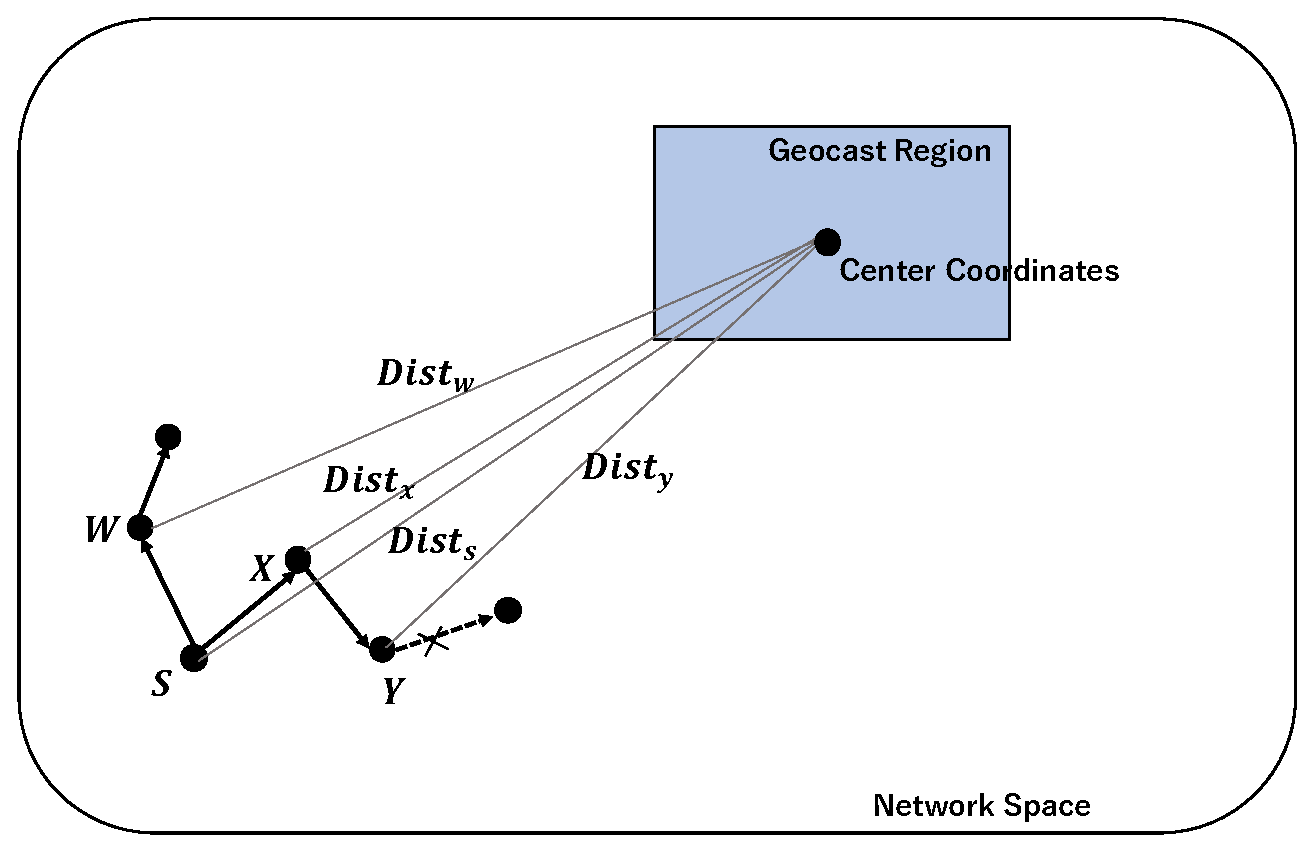
\includegraphics[width=100mm]{figures/Scheme2.eps}
	\caption{LBM:scheme2}
	\label{fig:scheme2}
\end{figure}

本研究では, 提案するOpportunistic routingを拡張し, Geocast routingにおいても有効であることを示す.



\section{Local optimum problem}
\label{local_optimum_problem}
\ref{Geographic}節で紹介したGeographic routingの既存研究では, 各送信ノードは自分より宛先ノードに近い隣接ノードの中から中継ノードとして最適なノードを1つ選択する. 同様に\ref{Opportunistic}節で紹介した多くのVANET用に設計されたOpportunistic routingにおいても, 各送信ノードは自分より宛先ノードに近い隣接ノードの中からRCSを選択する. しかし, 時には自分より宛先ノードに近い隣接ノードが存在しない場合が発生する. この問題をLocal optimum problem\cite{6}と呼ぶ. Local optimum problemは, 図\ref{fig:Local_optimum}のように建物による電波の遮断が起きやすい都市環境では発生確率が上昇する. したがって, 特にVANETにおいて自分より宛先ノードに近い隣接ノードから中継ノードを選択するタイプのルーチングでは, この問題を防ぐアプローチと発生した場合の対処法(Recovery strategy) の考案が必要である.

\begin{figure}[!ht]
	\centering
	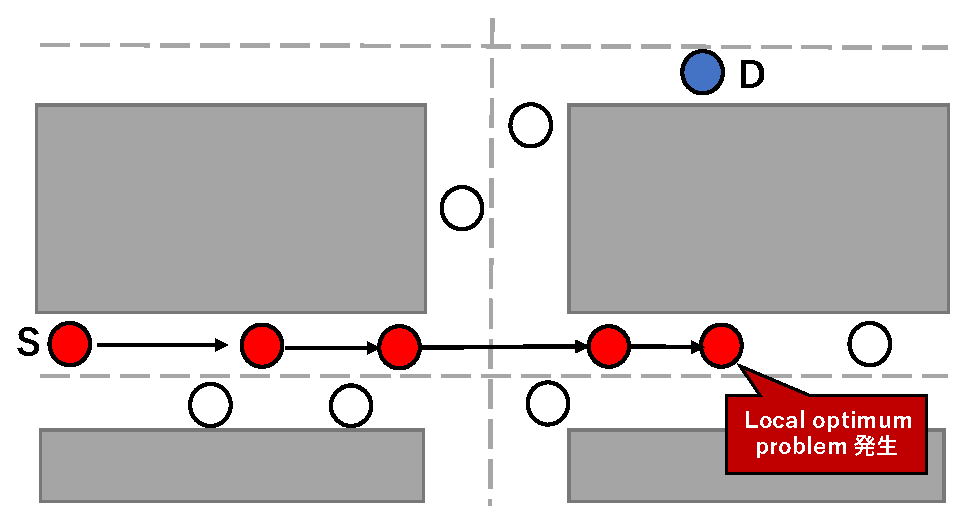
\includegraphics[width=130mm]{figures/Local_optimum_problem.eps}
	\caption{Local optimum problem}
	\label{fig:Local_optimum}
\end{figure}

\section{Recovery strategy}
前節で説明したLocal optimum problemがルーチング中に発生した場合, これに対処する中継戦略が必要となる. これをRecovery strategy\cite{28}と呼ぶ. Revovery strategyの基本モデルを図\ref{fig:Recovery}に示す. $N_{1}$でLocal optimum problemが発生する. 次に$N_{1}$は, 自身の位置情報をパケットに加えRecovery strategyを開始する. Recovery strategyは, Local optimum problemが発生したノード($N_{1}$)の位置より宛先に近いノードにパケットが到達するまで繰り返される. $N_{2}$までパケットが到達した場合$N_{2}$は$N_{1}$よりも宛先に近いため, 元の中継を開始する. 
  

\begin{figure}[!ht]
	\centering
	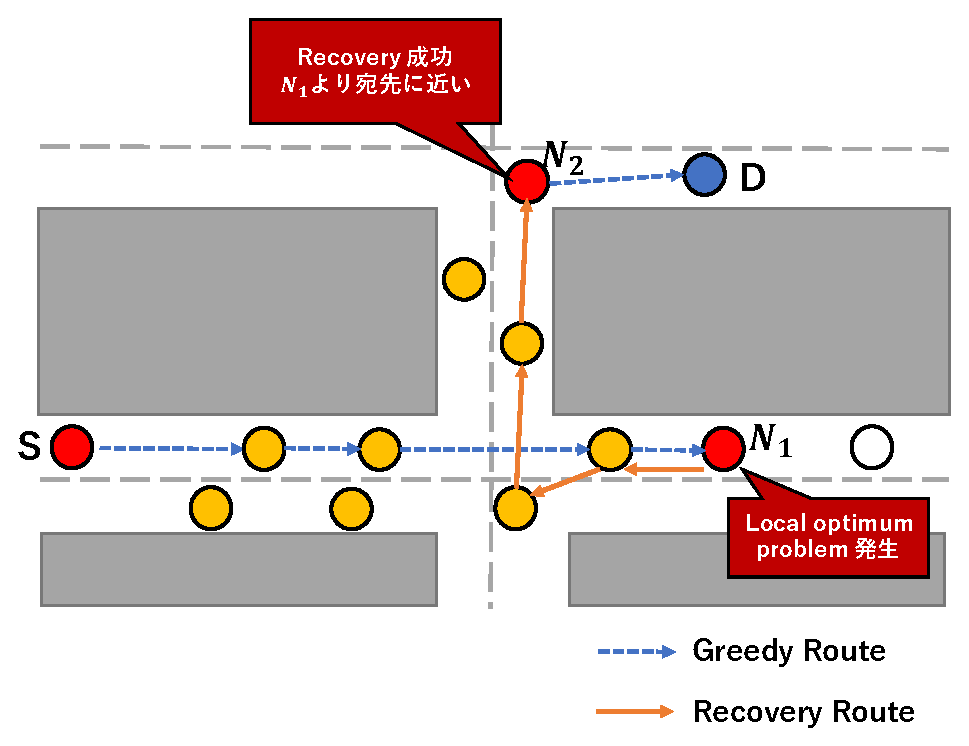
\includegraphics[width=130mm]{figures/basic-recovery.eps}
	\caption{Recovery strategy}
	\label{fig:Recovery}
\end{figure}

代表的なRecovery strategyとしてGreedy perimeter stateless routing(GPSR) \cite{6}の perimeter forwarding
と呼ばれるRecovery strategyが提案されている. perimeter forwardingの例を図\ref{fig:Perimeter}に示す. Perimeter fowardingではグラフ理論で古くからよく知られている右手の法則を使用する. この図では送信ノード$S$が宛先ノード$D$に最も近いためLocal optimum problemが発生している. この場合, 送信ノードは自分と宛先ノードを結んだ線から反時計回りに隣接ノードを探索し, 最初に発見したノードに対してパケットを送信する. Perimeter forwardingの2ホップ目以降では, 1ホップ前のノード(ノードxの場合はノードS)と自ノードを直線で結び, この直線から半時計回りに探索したノードに対してパケットを送信する. これを繰り返すことにより迂回ルートを構築することが可能になる. 
しかし, 右手の法則を使用する場合, すべてのエッジが交差していない必要がある. 例えば図\ref{fig:cross_link}のようなエッジ(リンク) の接続状態の場合(x → u → z → w → u → x)のようにループが発生する可能性がある. GPSRではループの原因となるクロスリンクを削除する方式が提案されているが, この方式は障害物が多く存在する都市環境ではネットワークの切断につながる可能性がある. したがって, Perimeter fowardingはVANETには適していない.




\begin{figure}[!ht]
	\centering
	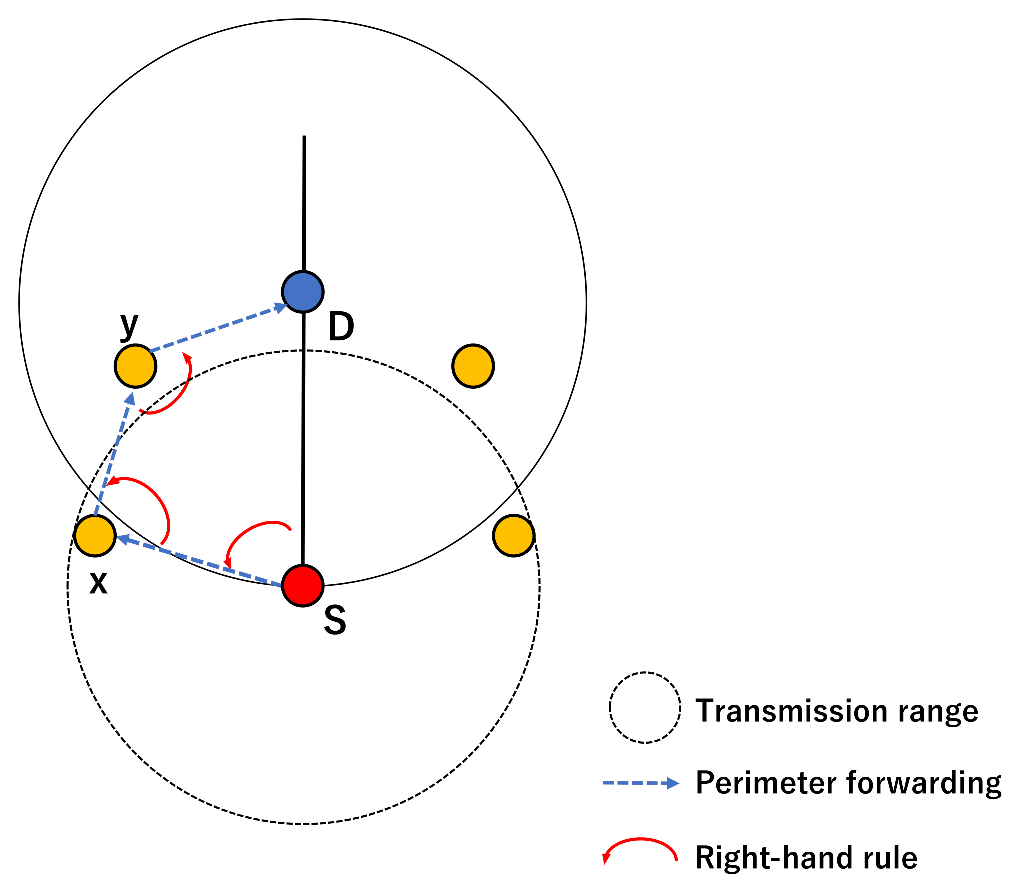
\includegraphics[width=130mm]{figures/Perimeter.eps}
	\caption{Perimeter fowarding}
	\label{fig:Perimeter}
\end{figure}

\begin{figure}[!ht]
	\centering
	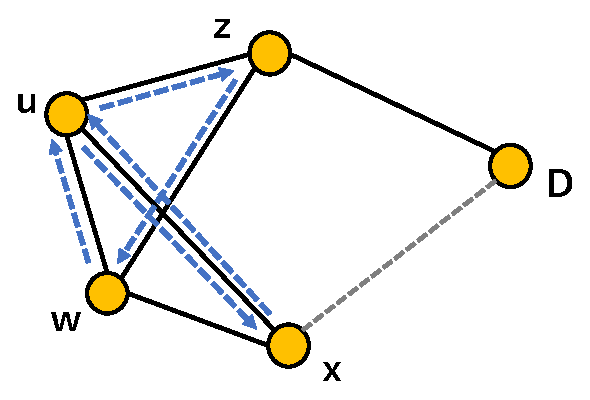
\includegraphics[width=100mm]{figures/cross-link.eps}
	\caption{ループが発生する例}
	\label{fig:cross_link}
\end{figure}

GPSRの問題点に対処するため, Greedy Perimeter Coordinator Routing (GPCR)\cite{7}が都市環境用に提案された. GPCRのRecovery strategyにおける主なアイデアは, Coordinatorと呼ばれる交差点に位置するノードを中継ノードとして最も優先して選択することである. GPCRのRecovery strategyの例を図\ref{fig:GPCR}に示す.
GPCRのRecovery strategyは, 右手の法則を使用した道路の選択と同一道路内の制限されたgreedy fowardingの2つの手順を繰り返し行う. 図\ref{fig:GPCR}ではLocal optimum problemが発生したノード$S$が転送する道路を選択し, 次の交差点を目指しgreedy fowardingを行う. パケットが交差点ノード$C_{1}$に到達すると, $C_{1}$は右手の法則を使用し, 転送する道路を選択する. この手順を繰り返す. GPCRでは, 各交差点にノードが存在する場合, GPSRのようにクロスリンクによるループは発生しない. しかし, 交差点ノードが存在しない場合ループが発生するという問題が生じる. この問題を解決するため, VANET cross Link Corrected Routing (VCLCR) \cite{29} が提案されている. VCLCRでは, 転送中の道路IDをパケットに格納することで, ルーチングループを検知し, クロスリンクを削除する. しかし, この方式ではパケットに格納すべきデータ量が増加することと, クロスリンクを削除するためのパケット数が増加してしまう問題がある. 

\begin{figure}[!ht]
	\centering
	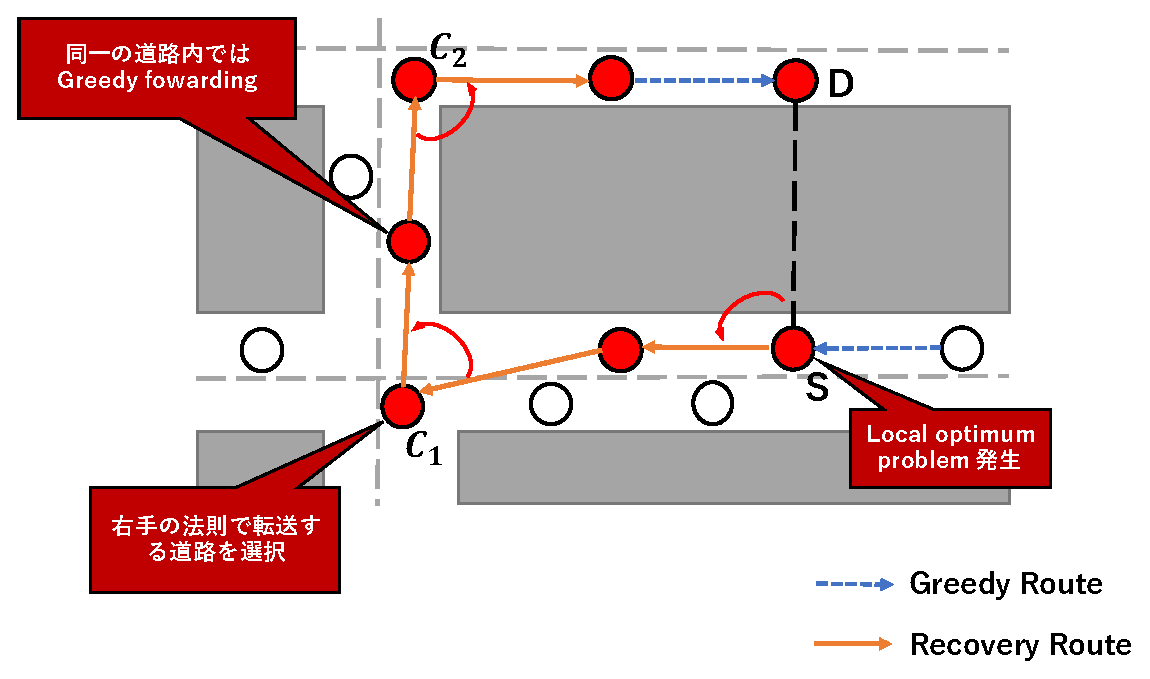
\includegraphics[width=130mm]{figures/GPCR.eps}
	\caption{GPCR}
	\label{fig:GPCR}
\end{figure}

Junction-Based Routing (JBR) \cite{JBR}のRecovery strategyでは, GPSRやGPCRのような右手の法則ではなく, 新たに最小角度法と呼ばれる手法を用いて中継ノードを選択する. JBRでは, 図\ref{fig:JBR}に示すように, 交差点ノードまでは従来の方式と同様にgreedy fowarding, 交差点ノードまでパケットが到達した場合, 交差点ノードは最小角度法に従って中継ノードを選択する. 図の例ではノードBが選択されている. 最小角度法の利点は, 右手の法則のようなループが起きないことである. 
しかし, JBRやGPCRのように交差点中心のRecovery strategyでは, 交差点ノードが存在しない場合アルゴリズムが機能しないという問題が発生する. また, JBRやGPCRなどの交差点中心のRecovery strategyを提案している既存研究の多くは, 建物によって電波が完全に遮断される仮定を基に, アルゴリズムが設計されている. これは現実的な仮定ではない. 
本研究ではこれらのRecovery strategyの問題に対処する新しいアルゴリズムを提案する. 
本節で紹介したプロトコルの特徴を表\ref{tab:Recovery}に示す.

\begin{figure}[!ht]
	\centering
	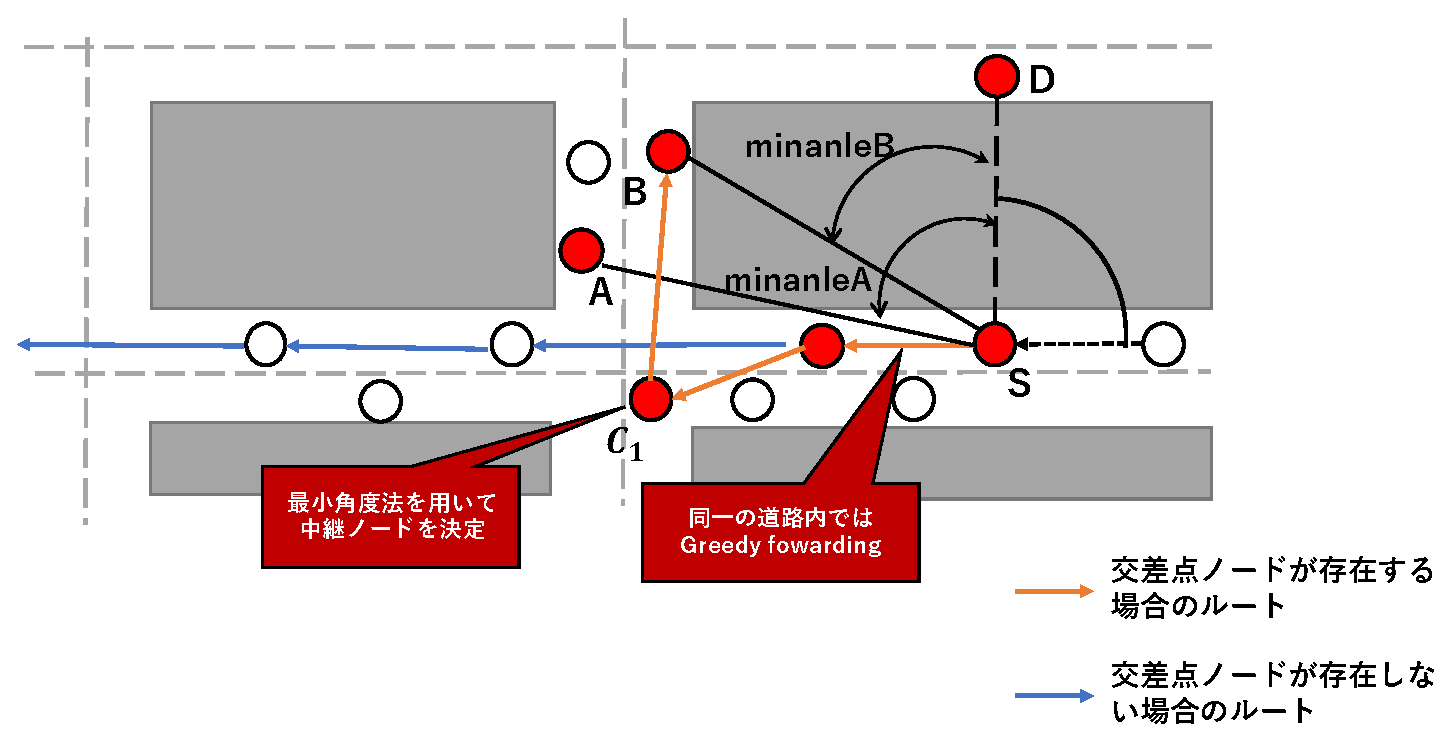
\includegraphics[width=140mm]{figures/JBR.eps}
	\caption{JBR}
	\label{fig:JBR}
\end{figure}

\begin{table}[h]
	\begin{center}
		\caption{Recovery strategy比較}
		\label{tab:Recovery}
		\centering
		\begin{tabular}{p{20mm}p{28mm}p{20mm}p{28mm}p{40mm}}
			\hline
			プロトコル & Recovery strategy & ループ回避 & 電波伝搬モデル & 問題点 \\
			\hline \hline
			GPSR & 右手の法則 & × & free space & クロスリンクによるループの発生. VANETのような都市環境には適していない.\\ 
			GPCR  & 右手の法則  & △ & building blocking &  交差点ノードが存在しないとループが発生する. \\
			VCLCR & 右手の法則  & 〇 & building blocking   &  ループを除去するためのパケット数, パケットのサイズが増大する. \\
			JBR & 最小角度法  & 〇 & building blocking   &  交差点ノードが存在しない場合, 宛先ノードから遠ざかる可能性がある. \\
			\hline
		\end{tabular}
	\end{center}
\end{table}



\chapter{LSGO}
\label{LSGO}
\section{概要}
LSGO\cite{18}はVANET用に設計されたOpportunistic routingでは代表的なものの1つである.
LSGOでは, 各ノードは自ノードのIDと現在の位置情報で構成されるHelloパケットを定期的にブロードキャストする. これにより各ノードは隣接ノードの情報を得ることができる.
送信ノード(ソースノードまたは任意の$i$ホップ目の中継ノード)は, Helloパケットで取得した情報に基づいて, 中継候補ノードセット:RCSの選定とそれらに優先順位を割り当て, データパケットをブロードキャストする. 各送信ノードはリンク品質と宛先までの距離の2つのメトリックに従って, RCSの優先順位を決定する. データパケットを受信した各ノードは, 自身のIDが含まれているかどうかを確認し, 含まれていない場合はパケットを破棄する. 含まれていた場合, 優先順位をチェックし, 優先度スケジューリングアルゴリズムに従ってパケットを再ブロードキャストするか否かを決定する.

\section{リンク品質の推定}
\label{link-quality}
LSGOでは, 各ノードがHelloパケットを定期的にブロードキャストし, それを用いてリンク品質ETXを推定する. Helloパケットは, 自ノードのID, X座標, Y座標で構成されている. ETXを算出するために, 各ノードは隣接ノードから最初にHelloパケットを受信した時間$t_{0}$を記録する. そして, 現在時刻を$t$, ウィンドウサイズを$w$(second), Helloパケットの送信間隔を$\tau$とすると, 予想伝送確率$r(t)$はウィンドウサイズ$w$で場合分けされ, 式(\ref{trans-prediction})で算出される.

\begin{equation}
	\label{trans-prediction}
	r(t) =\begin{cases}count(t, t_{0}), & 0 < t - t_{0} < 1,  \\ \frac{count(t,t_{0})}{(t-t_{0}) / \tau}, & 1 \leq t - t_{0} \leq w\\
		\frac{count(t - w,t)}{w / \tau}, &  t - t_{0} \geq w\\
	\end{cases}
\end{equation}


ウィンドウサイズ$w$は, $r(t)$を算出する際に, 現在時刻$t$より以前に取得したHelloパケットの有効期間である. 例えば, 現在時刻$t$=10(s), ウィンドウサイズ$w$=5(s)とすると, 時刻5(s)より古いHelloパケットの情報は$r(t)$を算出する際には用いない. $(t,t_{0})$ / $\tau$は, ウィンドウサイズの間に受信されるべきHelloパケット数であり, $count(t,t_{0})$は$t$ ~ $t_{0}$の期間中に実際に受信されたHello パケットの数である. \par
各隣接ノードとのリンクの非対称性は考慮せず, 一方向の予想伝送確率$r(t)$のみを使用してETXを計算する. 一方向伝送確率が$r(t)$であると仮定すると, リンク品質ETXは式(\ref{equ-intersection})で算出される.

\begin{equation}
	\label{equ-intersection}
	ETX = \frac{1}{  {r(t)}^{2}   } 
\end{equation}

\section{優先度スケジューリングアルゴリズム}

LSGOでは, タイマーベースの優先度スケジューリングアルゴリズムを使用する. このアルゴリズムでは, 最も優先度が高いノードが最初にパケットを送信する. ほかの候補ノードは, 優先順位の高いノードからのパケットを受信すると, 自身のパケットを破棄する. タイマーが期限切れになり, 自身より優先度の高いノードからのパケットを受信していない場合, 送信を開始する. LSGOは以下の式(\ref{pri-LSGO})によって, ノード$i$の優先度が算出される.

\begin{equation}
	\label{pri-LSGO}
	\frac{D_{sd} - D_{id}}{ETX_{i}^{2}} ,   D_{id} < D_{sd}
\end{equation}

$D_{sd}$は送信ノードから宛先ノードまでの距離, $D_{id}$は中継候補ノード$i$から宛先ノードまでの距離である.  $D_{id}$ \verb|<| $D_{sd}$の条件を満たさない場合は, 優先度の計算を行わずにRCSから除外する.
式(\ref{pri-LSGO})で算出された値が大きいほどノード$i$の優先順位が高くなる. 

\section{RCS選択アルゴリズム}
Opportunistic routingにおいてRCSに含まれるノード数が多い場合, バックアップリンクの数が多くなるためパケット到達率は向上するが, RCSに含まれるノード同士の協調(再ブロードキャストキャンセル)がされず冗長なパケットが増加する確率が高まるというトレードオフが存在する.  
このためLSGOでは, 信頼性を確保しながら, 送信回数を減らすためにRCSに含まれるノード数を最適化するアルゴリズムが提案されている.  
式(\ref{Min-Probability})を用いて各隣接ノードの優先順位を$p$ = 1,2.., $N$(1が最も優先順位が高い)とすると, $N$は次の条件を満たす必要があり, RCSに含まれるノードは1~$N$に制限される. 

\begin{equation}
	\label{Min-Probability}
	1 - \prod_{p=1}^N (1 - r_{p}(t))\geq R
\end{equation}

式(\ref{Min-Probability})における$r_{p}(t)$ (1$ \leqq $$p$$ \leqq $$N$)は, 送信ノードが保持する隣接ノード(優先順位$p$)に対する予想伝送確率である. 
式(\ref{Min-Probability})の左辺は送信ノードからのパケットを中継候補ノード1~$N$のいずれかのノードが受信すると予想される確率であり, 右辺$R$はその確率の閾値である. $R$が大きいほど, RCSに含まれるノード数が増加し, 小さくなるほどRCSに含まれるノード数が減少する. 車両密度が小さい場合や送信ノードと各隣接ノード間の予想伝送確率が低い場合, 式(\ref{Min-Probability})満たすことができない場合がある. その場合, $D_{id}$ \verb|<| $D_{sd}$の条件を満たすすべての隣接ノードがRCSとして選択される. また, 送信ノードと各隣接ノードとの予想伝送確率が高い場合, RCS数$N$は小さくなるため, 信頼性を確保しながら, 最低限のRCS数を選択することができる. 


\section{シャドウイングとRCS数の影響}
\label{LSGO_evaluation}

本節では, シャドウイングによる電波減衰が起きやすい都市環境において, RCSに含まれるノード数がどのように通信性能に影響を与えるのか, LSGOのRCS選択アルゴリズムは有効なのかを調査する.
また, シャドウイングによる電波減衰が起こる場合と起こらない場合とでのLSGOの通信性能に与える影響を調査する.

\subsection{シミュレーション設定}
シミュレーションパラメータを表\ref{tab:parameter}, シミュレーションシナリオを図\ref{fig:Scenario}に示す. シミュレーションシナリオは交通流シミュレータのSUMO\cite{27}を使用して作成した. シミュレーション開始時に, ランダムな送信ノードと宛先ノードがそれぞれ10台ずつ割り当てられ, 通信を開始する. 各交差点には信号機を配置し, 図の灰色の領域に建物を配置した. 
Ns-3の電波伝搬モデルとしてシャドウイングモデルであるObstacle shadowing model\cite{20}を使用した. シャドウイングによる伝搬損失$L_{s,o}$は各壁による損失と建物の貫通距離(m)に基づいて式(\ref{shadowing})で算出される.

\begin{equation}
	\label{shadowing}
	L_{s,o} = \alpha n  + \beta d_0
\end{equation}

シャドウイングモデルには2つのパラメータが存在する. $\alpha$は電波が通過する壁あたりの減衰(db), $\beta$は電波が通過する建物の貫通距離あたりの減衰(db)である. また, $n$は貫通した建物の壁の数であり, $d_{o}$は建物の貫通距離(m)である.
本シミュレーションでは, $\alpha$= 10 dB and $\beta$= 0.4 dB で評価を行った. 

\begin{figure}[!ht]
	\centering
	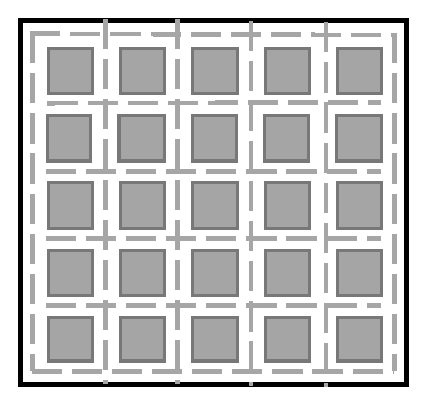
\includegraphics[width=70mm]{figures/Scenario.eps}
	\caption{シミュレーションシナリオ}
	\label{fig:Scenario}
\end{figure}

\begin{table}[!ht]
	\begin{center}
		\caption{シミュレーションパラメータ}
		\label{tab:parameter}
		\begin{tabular}{|l|l|lll}
			\cline{1-2}
			Network Simulator    & Ns-3 (v3.30) &  &  &  \\ \cline{1-2}
			Traffic Simulator    & SUMO &  &  &  \\ \cline{1-2}
			Simulation area    & 1000m × 1000 m   &  &  &  \\ \cline{1-2}
			Mobility model     & Random mobility &  &  &  \\ \cline{1-2}
			Transmission range & 250 m            &  &  &  \\ \cline{1-2}
			Number of vehicles & 200, 300, 400      &  &  &  \\ \cline{1-2}
			Radio propagation model    & obstacle shadowing model\cite{20}&  &  &  \\ \cline{1-2}
			MAC Layer     & 802.11p &  &  &  \\ \cline{1-2}
			Packet Size & 512 byte       &  &  &  \\ \cline{1-2}
			Simulation Time & 30 s      &  &  &  \\ \cline{1-2}
			hello interval & 1 s      &  &  &  \\ \cline{1-2}
			Window size w  & 10 s      &  &  &  \\ \cline{1-2}
			%Number of relay candidate nodes  & 5       &  &  \\ \cline{1-2}
			shadowing parameter $\alpha$  & 10db      &  &  &  \\ \cline{1-2}
			shadowing parameter $\beta$    & 0.4db &  &  \\ \cline{1-2}
		\end{tabular}
	\end{center}
\end{table}

\subsection{評価項目}
\label{evaluation_item}
本シミュレーションでは, LSGOの通信性能を評価するためパケット到達率(PDR), エンドツーエンド遅延(Delay), オーバーヘッド(Overhead)の3つの評価項目で評価した. PDR, Delay, Overheadの算出式をそれぞれ式\ref{PDR}, \ref{delay}, \ref{overhead}に示す.

\begin{equation}
	\label{PDR}
	PDR = \frac{D_{recv}}{  S_{sent}  } \times 100
\end{equation}

ここで, PDRはソースノード(データパケットを一番初めに生成したノード)から宛先ノードに送信されるパケットの到達率を表す. $S_{sent}$はソースノードが送信した合計パケット数を表し, $D_{recv}$は宛先ノードが受信した合計パケット数を表す.

\begin{equation}
	\label{delay}
	Delay = \frac{\sum_{i=1}^{N}ED_i}{N}
\end{equation}

ここでエンドツーエンド遅延(秒)は, ソースノードがパケットを送信してから宛先ノードに到達するまでにかかる平均時間を表す. $ED_i$は, 宛先ノードが正常に受信したパケット$i$ (1$ \leqq $$i$$ \leqq $$N$) が, ソースノードの送信から宛先ノードに到達するまでにかかる時間を表す. 
$N$は宛先ノードが正常に受信したパケット数を表す.

\begin{equation}
	\label{overhead}
	Overhead = \frac{N_{sent}}{  D_{recv}  }
\end{equation}

ここでオーバーヘッドは, 1つのデータパケットを宛先ノードに届けるためにどれだけのパケット数を費やしたかを表す. $N_{sent}$はネットワーク全体における各ノードが送信した合計パケット数を表す.

\subsection{RCS数の影響}
本シミュレーションでは, RCSに含まれるノード数が通信性能にどのように影響するのかを評価した.
シャドウイングパラメータ$\alpha$ = 10, $\beta$ = 0.4, ノード数は400に設定した.
図\ref{fig:RCS-PDR}, \ref{fig:RCS-delay}, \ref{fig:RCS-overhead}は, RCS数を変化させたときのパケット到達率, エンドツーエンド遅延, オーバーヘッドを示している. RCS\_LSGOは, RCS数をLSGOのアルゴリズムに従って決定した場合の取得データを示している. 今回のシミュレーションでは, 式\ref{Min-Probability}の閾値$R$は, RCS数が最も多くなる1.0に設定した. RCS\_1~5はRCS数を1~5個に設定した時の取得データを示している. また, RCS\_1~5の時のRCS数は最大値であり, 各送信ノードより宛先ノードに近いノードが設定したRCS数より少ない場合, 隣接するすべてのノードがRCSに含まれる.
\par
\vspace{5mm}
\noindent
\textbf{パケット到達率(PDR)}
\vspace{5mm}


図\ref{fig:RCS-PDR}が示す通り, RCS数が増加するほどパケット到達率が向上している. これはRCS数が多いほど, RCSに含まれるノードのいずれかにパケットが到達する確率が上昇するからである. また, 本シミュレーションシナリオとobstacle shadowing modelを用いて評価した場合, LSGOのRCS選択アルゴリズムの性能が低いことがわかる. LSGOのRCS選択アルゴリズムは予想伝送確率を使用して設計されており, 予想伝送確率はHelloパケットの受信履歴から計算される. しかし, 実際のHelloパケットはデータパケットよりもデータサイズが小さいため, データパケットより高確率で受信される. これがこのアルゴリズムの性能低下の原因だと推測される.

\begin{figure}[!ht]
	\centering
	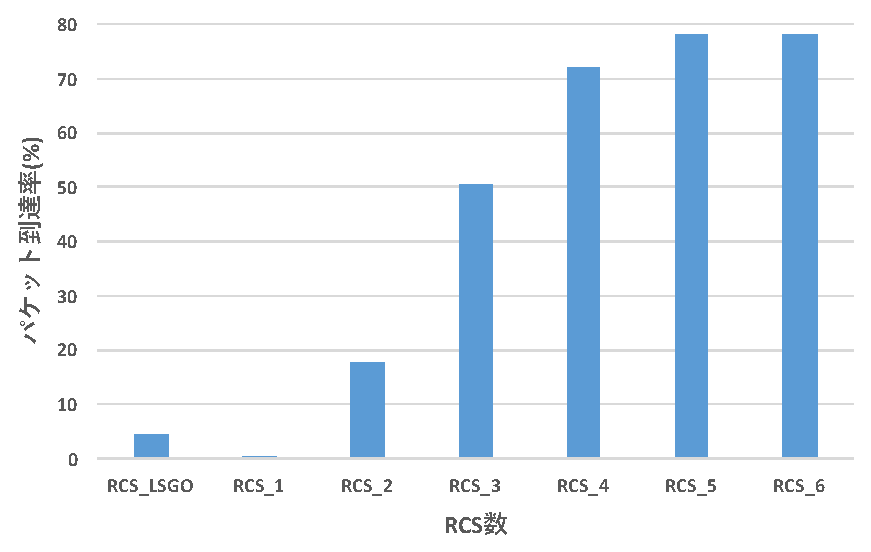
\includegraphics[width=110mm]{figures/RCS_PDR.eps}
	\caption{RCS数の変化にともなうPDR}
	\label{fig:RCS-PDR}
\end{figure}

\par
\vspace{5mm}
\noindent
\textbf{エンドツーエンド遅延}
\vspace{5mm}

図\ref{fig:RCS-delay}が示す通り, RCS数が増加するほど, 遅延は増加している. これは2つの理由が推測される. 1つ目は, RCS数が少ない場合, ソースノードと宛先ノードの距離が近い場合のみ宛先ノードが正常にパケットを受信したからである. 図\ref{fig:RCS-hop}に, 送信ノードから宛先ノードまで正常に到達したパケットの平均ホップ数を示す. RCS数が少ない場合, ホップ数が減少していることがわかる. これはRCS数が少ない時には, 送信ノードと宛先ノードの距離が近い場合に限り, 正常にパケットが到達したことを示している.
2つ目は, RCS数が多いほど, 優先順位が低い中継候補ノードのみパケットを受信した場合, 優先順位の低いノードほど待ち時間(中継タイマー)が長いからである.


\begin{figure}[!ht]
	\centering
	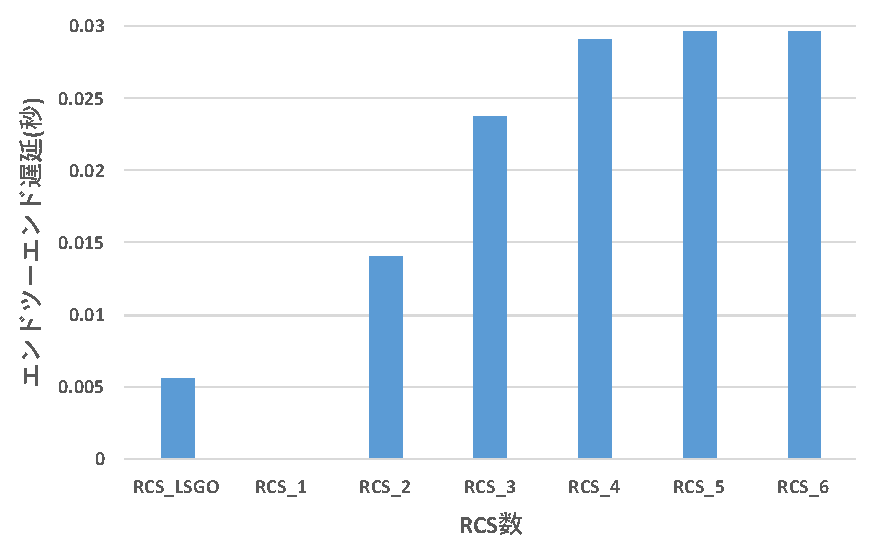
\includegraphics[width=110mm]{figures/RCS_Delay.eps}
	\caption{RCS数の変化にともなうエンドツーエンド遅延}
	\label{fig:RCS-delay}
\end{figure}

\begin{figure}[h]
	\centering
	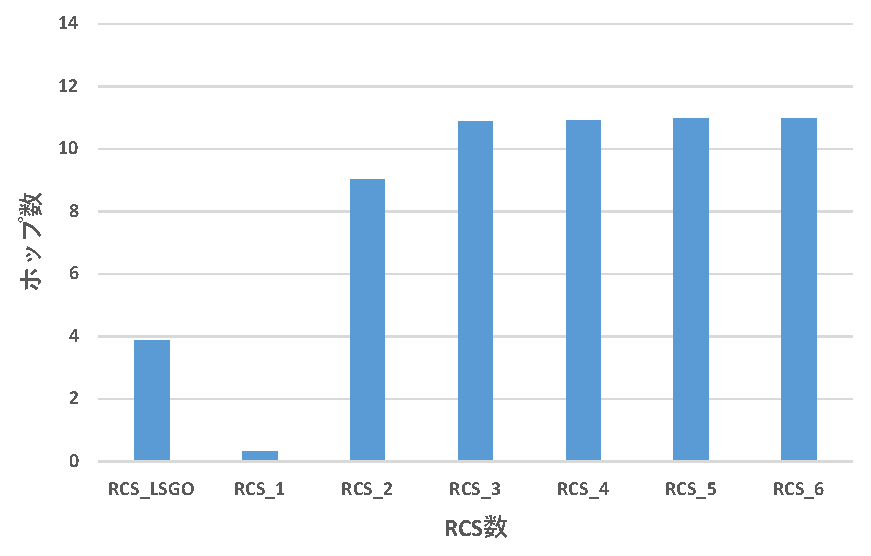
\includegraphics[width=110mm]{figures/RCS_Hop.eps}
	\caption{RCS数の変化にともなうホップ数}
	\label{fig:RCS-hop}
\end{figure}



\par
\vspace{5mm}
\noindent
\textbf{オーバーヘッド}
\vspace{5mm}

図\ref{fig:RCS-overhead}が示す通り, RCS数が増加するほど, オーバーヘッドが減少している. これはRCSが増加するほど, ネットワーク全体における各ノードが送信した合計パケット数は増加しているが, 宛先ノードが正常に受信したパケット数も増加したためである. また, ホップ数が著しく低いRCS数が1の場合を除き, RCS数が増加するほどオーバーヘッドが減少しているが, RCS数が5から6になるにかけて少し増加している. これは, 5から6にかけて宛先が正常に受信したパケット数に差がないのに対して, ネットワーク全体における各ノードが送信した合計パケット数が増加しているからである. したがって, 本シミュレーションではRCS数5の場合が最も効率的であったといえる. 

\begin{figure}[!ht]
	\centering
	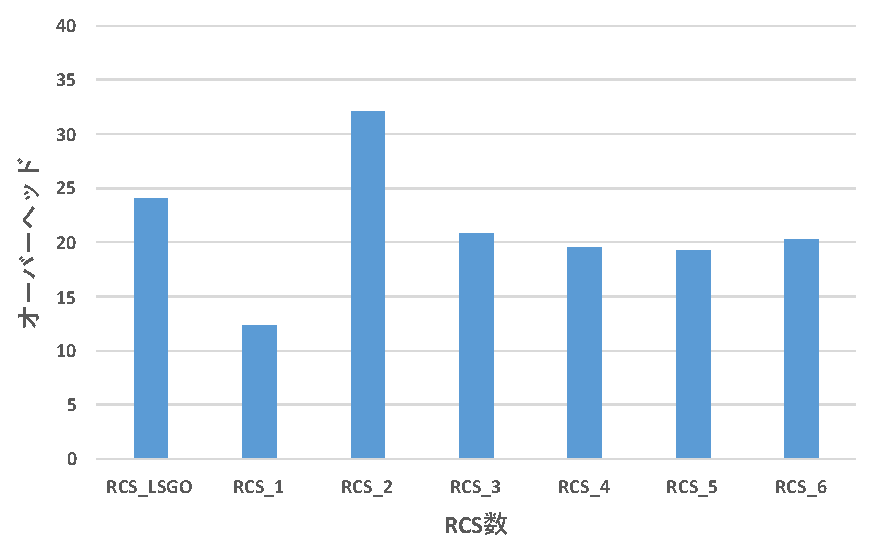
\includegraphics[width=110mm]{figures/RCS_Overhead.eps}
	\caption{RCS数の変化にともなうオーバーヘッド}
	\label{fig:RCS-overhead}
\end{figure}



\subsection{シャドウイングの影響}
本シミュレーションでは, 建物のシャドウイングによる電波の減衰が起こる場合のLSGOの通信性能に与える影響を評価した.
またRCS数は5に設定した.

\par
\vspace{5mm}
\noindent
\textbf{パケット到達率}
\vspace{5mm}

図\ref{fig:LSGO-PDR}は, ネットワークシミュレーションでシャドウイングの影響を考慮した場合としない場合とでの, パケット到達率を示している.
シミュレーションでシャドウイングを考慮した場合, 全てのノード数においてパケット到達率が減少している. これは, シャドウイングによる電波減衰が原因だと推測される.



\begin{figure}[!ht]
	\centering
	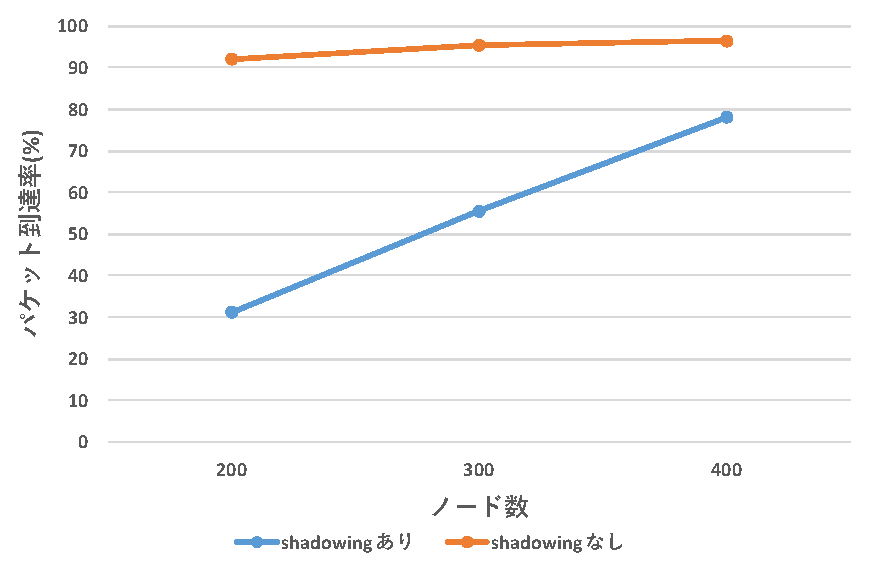
\includegraphics[width=110mm]{figures/LSGO_PDR.eps}
	\caption{パケット到達率 シャドウイングの有無}
	\label{fig:LSGO-PDR}
\end{figure}

\par
\vspace{5mm}
\noindent
\textbf{エンドツーエンド遅延}
\vspace{5mm}

図\ref{fig:LSGO-delay}は, はネットワークシミュレータでシャドウイングの影響を考慮する場合としない場合とでのエンドツーエンド遅延(秒)を
示している. シミュレーションでシャドウイングを考慮した場合, 全てのノード数においてエンドツーエンド遅延が増加している. これはシャドウイングによる電波減衰が起こり, 建物を通過するパケットが届きにくくなることで,  ソースノードと宛先ノードを直線的に結ぶような経路が形成することが難しくなったことが原因だと考えられる.

\begin{figure}[!ht]
	\centering
	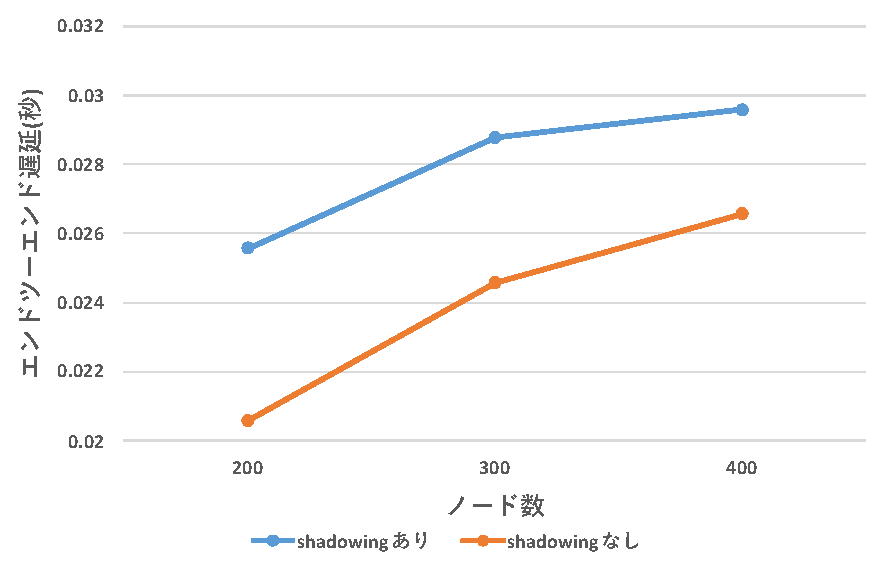
\includegraphics[width=110mm]{figures/LSGO_delay.eps}
	\caption{エンドツーエンド遅延 シャドウイングの有無}
	\label{fig:LSGO-delay}
\end{figure}


\par
\vspace{5mm}
\noindent
\textbf{オーバーヘッド}
\vspace{5mm}

図\ref{fig:LSGO-overhead}は, ネットワークシミュレータでシャドウイングの影響を考慮した場合としない場合とでのオーバーヘッドを示している.
シミュレーションでシャドウイングを考慮した場合, すべてのノード数においてオーバーヘッドが増加している. これは2つの理由が推測される.
1つ目は, シャドウイングによる電波減衰が起こり, 建物を通過するパケットが届きにくくなることで,  ソースノードと宛先ノードを直線的に結ぶような経路が形成することが難しくなったため, ホップ数が増加したと推測される. 
2つ目は, opportunistic routingにおいて送信ノードから指定されたRCSに含まれるノード同士が自分より優先度の高いノードからのパケットを建物による電波減衰によって, 受け取れない確率が増加し, 再転送がキャンセルされていないことが原因だと推測される.


\begin{figure}[!ht]
	\centering
	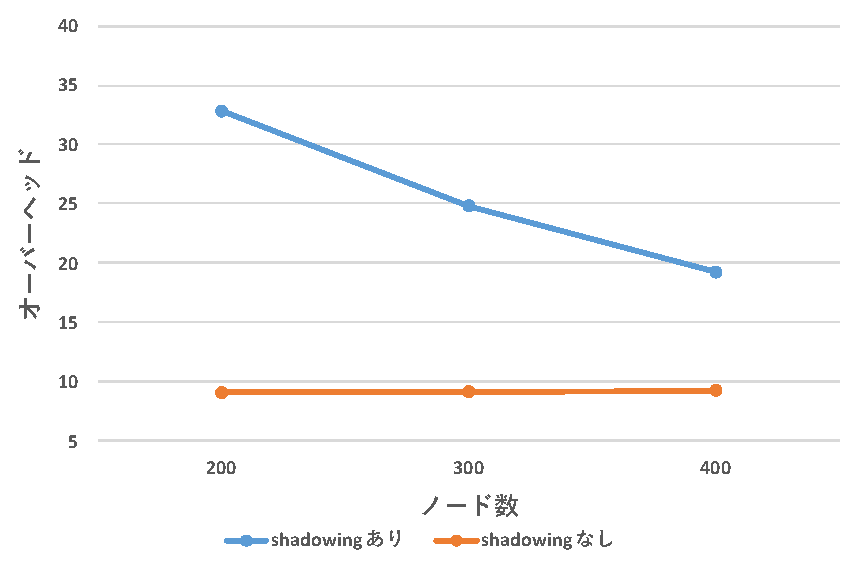
\includegraphics[width=110mm]{figures/LSGO_overhead.eps}
	\caption{オーバーヘッド シャドウイングの有無}
	\label{fig:LSGO-overhead}
\end{figure}


\subsection{LSGOの問題点}
本節では, LSGOの中継戦略の問題点について考察する. LSGOでは, 中継候補ノードの優先順位をあて先ノードまでの近さとリンク品質を基に決定する. 問題のあるシチュエーションの一例を図\ref{fig:LSGO-problem}に示す. 

\begin{figure}[!ht]
	\centering
	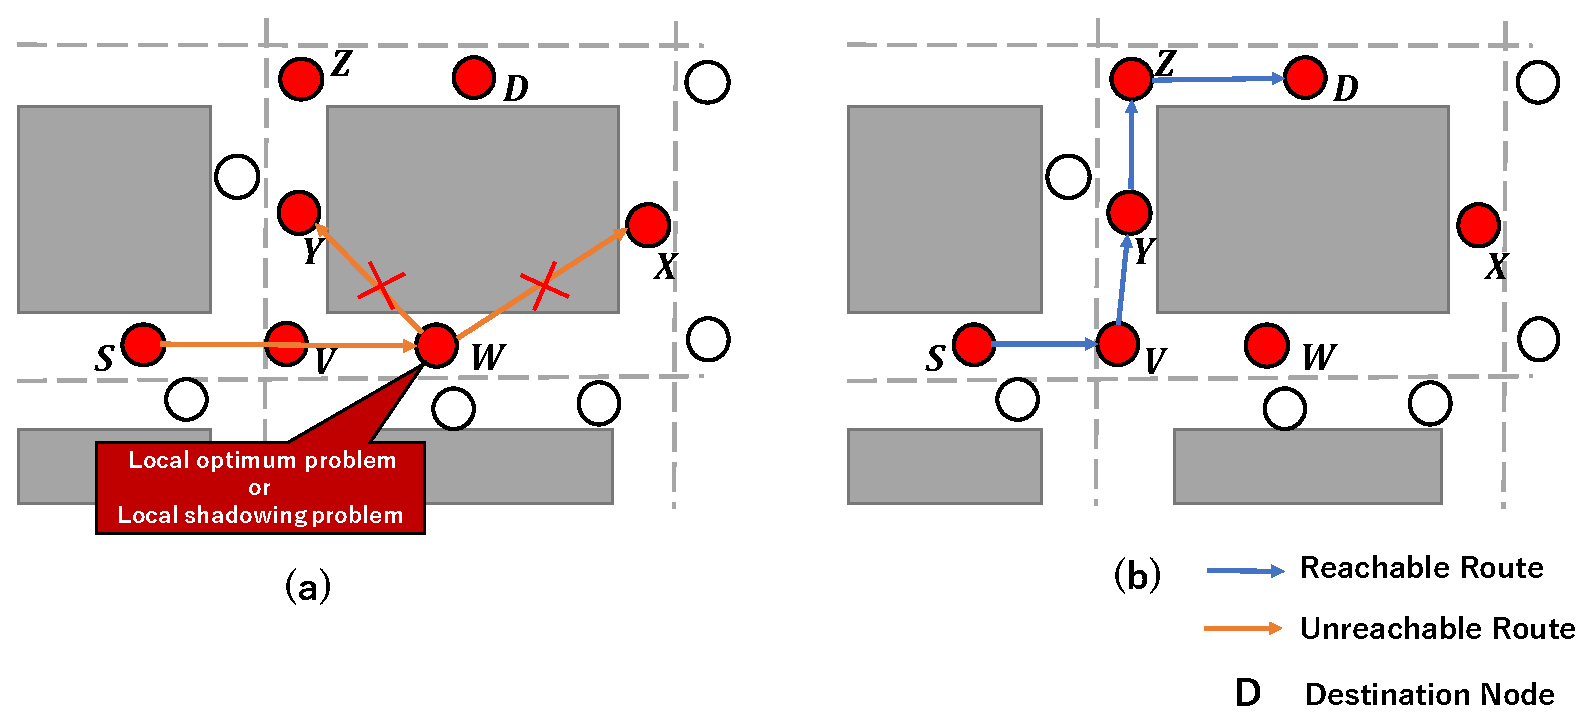
\includegraphics[width=160mm]{figures/LSGO_problem.eps}
	\caption{中継戦略の問題点}
	\label{fig:LSGO-problem}
\end{figure}

図(a)のように送信ノード$S$が, ノード$W$を最も優先度の高い中継ノードとして選択した場合を考える. この場合, ノード$W$に続く中継ノード(ノード$W$より宛先に近いノードを選択)は, シャドウイングによりリンク品質が良くないノード$X$と$Y$のみとなる. この問題をLocal shadowing problemと呼ぶ. また, シャドウイングの強度が強い場合, $X$と$Y$のリンクが完全に遮断されている場合が考えられる. この場合, \ref{local_optimum_problem}節で紹介したLocal optimum problemが発生する. これらのことから, LSGOの中継戦略は, Local shadowing problemやLocal optimum problemに陥る可能性が高いことがわかる. この問題は, 図\ref{fig:LSGO-problem}(b)に示すように, ノード$V$のような交差点ノードを中継ノードとして選択することで回避することができる. 





\chapter{車両位置とリンク状態を考慮した地理的opportunistic routing}
\label{Proposed}
\section{概要}
本研究では, 以下の3つを提案する. \par
\textbf{1. シャドウイングを考慮したOpportunistic routing(SIGO)} \par
\textbf{2. シャドウイングを考慮したOpportunistic recovery strategy(ORS)} \par
\textbf{3. 1のoppotrunistic routingを基に拡張したgeocast routing} \par

1ではLSGOの問題点を解決するOpportunistic routingを提案する. 性能評価では, LSGOとの比較を行った. 2では, 既存Recovery strategyの問題を解決するOpportunistic Recovery strategy提案する. 提案するRecovery strategyと比較手法としてJBRをSIGOのRecovery strategyとして加え比較を行った.
3では, SIGOとLSGOをそれぞれgeocast routingに拡張し, それぞれの比較を行った.

\section{前提条件}
SIGOでは, 以下のような仮定と定義をおいている. 

\begin{itemize}
	\item  \textit{road segment} : 2つの交差点を結ぶ道路の一部分. (交差点は含めない)
	\item \textit{ソースノード} : データパケットを生成し, 最初にデータパケットをブロードキャストするノード. 
	\item  \textit{送信ノード} : ソースノードまたは任意の$i$ホップ目の中継ノード.
	\item  \textit{RCS(Relay candidate nodes set)} : Opportunistic routingにおいて, 各送信ノードが選択する中継候補ノードの集合. 
	\item  \textit{中継候補ノード} : RCSに含まれるノードの1つを表す. 
	\item  \textit{LSN} : Local optimum problemを検知し, 初めにrecovery strategyを開始するノード.
	\item  \textit{PLSN} : LSNの1ホップ前のノード(LSNはPLSNからパケットを受信した).
	\item すべてのノードがGPSを搭載しており, デジタルマップを利用できることを想定する. 
	\item 各ノードは隣接ノードから定期的に受信するHelloパケットの情報と, デジタルマップの情報を用いて, 隣接ノードが存在するroad segmentや交差点を判別する.
	\item 宛先ノードの位置情報は, 何らかの位置情報サービスを利用することを想定する. 
\end{itemize}




\section{SIGO: Shadowing-based Intersection Geographic Opportunistic Routing}
\label{SIGO}

本研究では, shadowing-based intersection geographic opportunistic routing(SIGO)という, シャドウイングを考慮したOpportunistic routingを提案する. SIGOでは, 中継ノードの優先度を決定するメトリックとして, 宛先ノードまでの距離, リンク品質に加え, 交差点ノードを優先する指標である$IRI$(intersection relay index)を用いる. 最初の2つのメトリックは, \ref{LSGO}章で紹介したLSGOと同様の方法で算出する. SIGOでは, LSGOと同様に各ノードが定期的にHelloパケットをブロードキャストする. 送信ノードは宛先ノードにパケットを届けるために, Helloパケットで収集した情報に基づいて, RCSの選定とRCSに含まれるノードの優先度情報を含むデータパケットをブロードキャストする. RCSの優先度は後述するアルゴリズムに従って, 決定する. データパケットを受信した各ノードは, パケットに自身のIDが含まれているかどうかを確認し, 含まれていない場合はパケットを破棄する. 含まれている場合, ノードは自身の優先度をチェックし\ref{SIGO_priority}節で説明する優先度スケジューリングアルゴリズムに従ってパケットを再ブロードキャストするか否かを決定する.

\subsection{パケットフォーマット}

SIGOでは, 各ノードが定期的にHelloをブロードキャストして, 隣接ノードのリンク品質と位置を把握する. Helloパケットのフォーマットを図\ref{fig:hello_packet}に示す.

\begin{itemize}
	\item $ID$: Helloパケットを送信するノードの$ID$
	\item $X$: Helloパケットを送信するノードの$x$座標.
	\item $Y$: Helloパケットを送信するノードの$y$座標.
\end{itemize}


\begin{figure}[!ht]
	\centering
	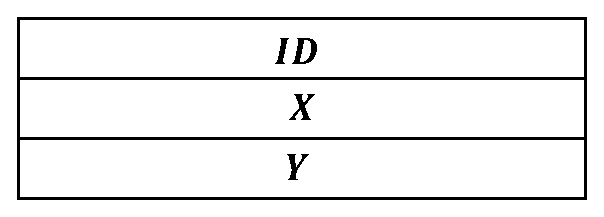
\includegraphics[width=70mm]{figures/hello_packet_format.eps}
	\caption{Helloパケットフォーマット}
	\label{fig:hello_packet}
\end{figure}

データパケットのフォーマットを図\ref{fig:SIGO_packet}に示す. SIGOでは制御パケットを使用しないため, 各中継候補ノードに割り当てられた優先度情報がデータパケットに含まれる.

\begin{itemize}
	\item $SourceId$: ソースノードのID.
	\item $DstId$: 宛先ノードのID.
	\item $Dst_x Pos$: 宛先ノードの$x$座標.
	\item $Dst_y Pos$: 宛先ノードの$y$座標.
	\item $ID_i$: 中継候補ノードの優先度$i$. $i$ = 1, 2, 3, ...(数字が低いほど優先順位が高い) 
	\item $Data$: ペイロード部.
\end{itemize}


\begin{figure}[!ht]
	\centering
	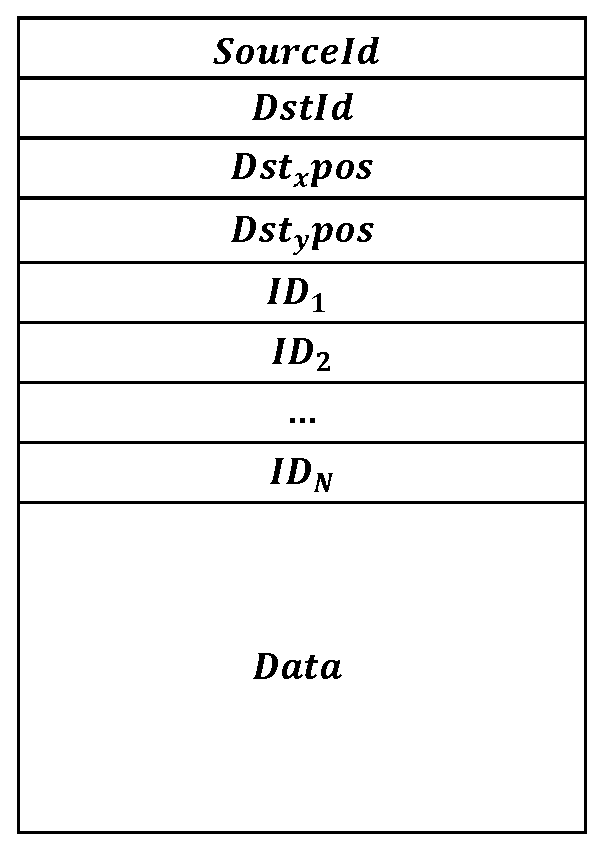
\includegraphics[width=70mm]{figures/SIGO_packet_format.eps}
	\caption{SIGOデータパケットフォーマット}
	\label{fig:SIGO_packet}
\end{figure}


\subsection{Intersection Relay Index (IRI)}
SIGOでは, 各送信ノードは以下の2つの条件を満たした場合$IRI$を算出する.

\begin{itemize}
	\item 送信ノードよりも宛先ノードに近い交差点ノードが存在する.
	\item 送信ノードが存在するroad segmentに隣接する交差点に交差点ノードが存在する.
\end{itemize}

$IRI$は以下の手順で算出する. \par
\textbf{手順1: 最も宛先ノードに近いroad segment(closest road segment)の選定.}
送信ノードは, 自分より宛先ノードに近い隣接ノードが存在するroad segmentの中で, 宛先ノードに最も近いroad segmentを1つ選択する. 図\ref{fig:closest_road_segment}に示すように, 最も宛先ノードに近いroad segmentの算出には, 各road segmentの中心座標を用いる. 

\textbf{手順2: closest road segmentへの予想伝送確率の算出.} 送信ノードはclosest road segmentに位置するノードの中で, 少なくとも1つのノードに到達する予想伝送確率$R_p$を式\ref{Rp}で算出する.

\begin{equation}
	\label{Rp}
	R_p = 1 - \prod_{k=1}^N (1 - r_{k}(t))
\end{equation}

ここで, $r_k(t)$は, closest road segmentに存在するノード$k$ (1 $\leq$  $k$ $\leq$ $N$)の予想伝送確率である. 予想伝送確率は, \ref{link-quality}と同様の方法で算出する. $N$はclosest road segmentに存在するノード数を表す. 

\begin{figure}[!ht]
	\centering
	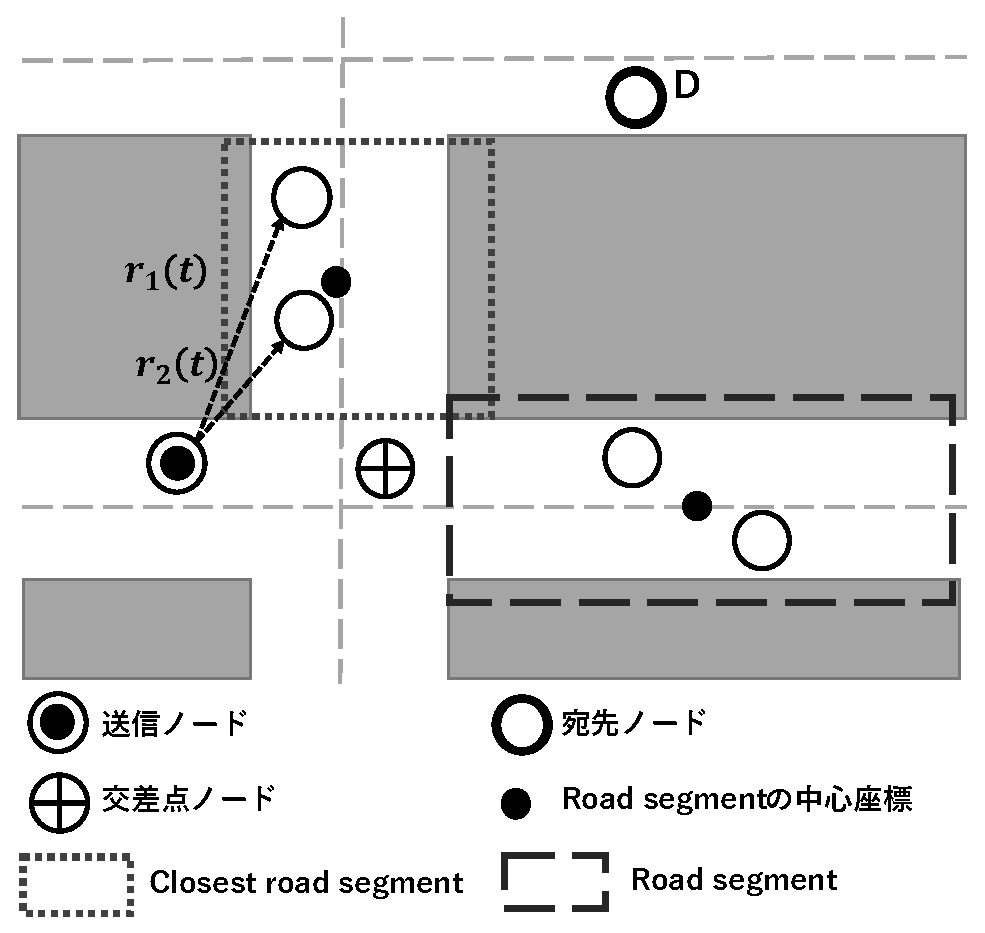
\includegraphics[width=120mm]{figures/closest_road_segment.eps}
	\caption{Closest road segment}
	\label{fig:closest_road_segment}
\end{figure}

\textbf{手順3: $IRI$の算出.} 手順2で算出した$R_p$を用いて, 隣接交差点ノード$i$の$IRI_i$を式\ref{IRI}で算出する.

\begin{equation}
	\label{IRI}
	IRI_i =  \alpha\frac{\theta_i}{R_p}, \theta_i \geq 45
\end{equation}

ここで, $\theta_i$は図\ref{fig:angle}に示すように, 送信ノードと宛先ノードを結ぶ直線と, 送信ノードと交差点ノード$i$を結ぶ直線のなす角度である. $\theta_i$が大きくなるほど, $R_p$が小さくなるほど, $IRI_i$は大きくなる. 
$\alpha$ ($\alpha$ \verb|>| 0) は, $IRI_i$の重み付け係数である. $IRI_i$が大きくなるほど, 送信ノードは高い確率で交差点ノード$i$をRCSに含み, 高い優先度を与える確率が増加する. 提案方式では$R_p$が小さい場合, 交差点ノードが優先される確率が高まる. これは, 交差点ノードを介してclosest road segmentに存在するノード群にパケットを届けることが目的である. また, $\theta_i$ ($\theta_i$ \verb|<=| 90 )が大きい場合, 送信ノードは高い確率で交差点ノード$i$をRCSに含み, 高い優先度を与える確率が増加する.
これは, $\theta_i$が大きいとき, 宛先までの距離とリンク品質で優先度を算出すると図\ref{fig:aim_SIGO}のような優先順位になる確率が高まる. この場合, Local optimum problemになる確率が増加する. したがって, これを防ぐために提案方式では$\theta_i$が大きくなるほど, 交差点ノードの優先度が増加するように設計した.
また, $\theta_i$が小さい場合交差点ノードが優先されると, ホップ数が増加し通信性能が低下する問題が発生する. 
そのため, 提案方式では$\theta_i$が45より大きい場合のみ, $IRI_i$の優先度を算出する.


\begin{figure}[!ht]
	\centering
	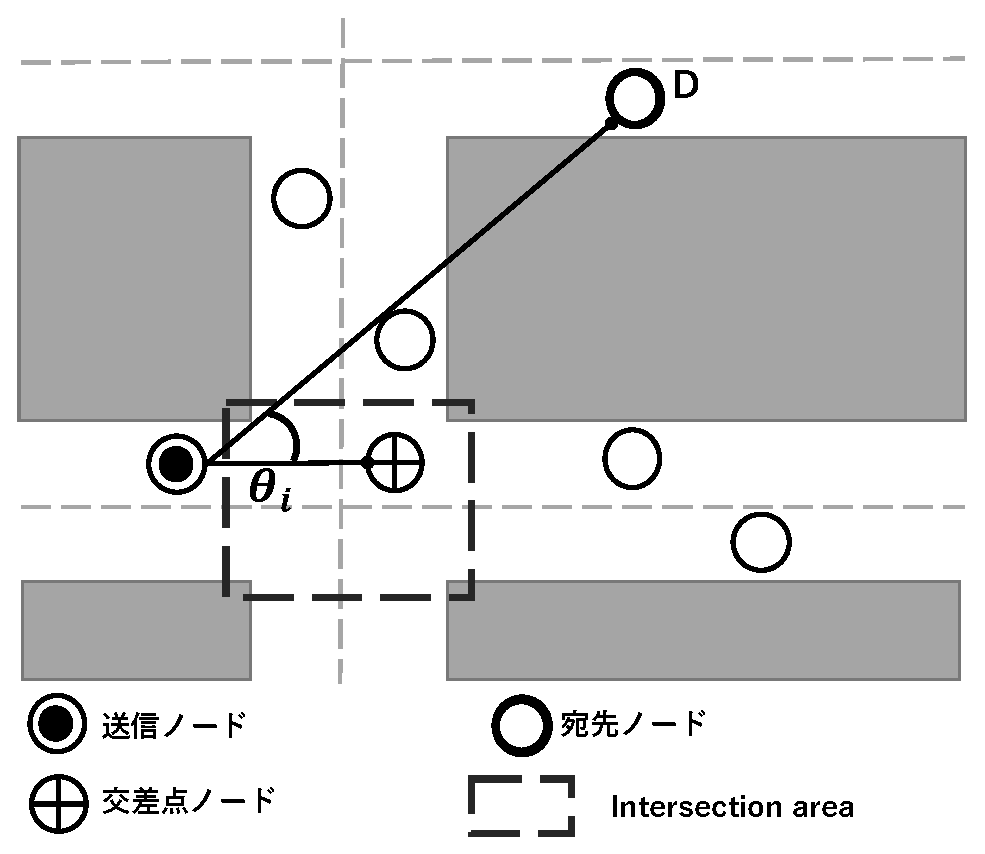
\includegraphics[width=120mm]{figures/angle.eps}
	\caption{$\theta_i$に制限を与える目的}
	\label{fig:angle}
\end{figure}

\begin{figure}[!ht]
	\centering
	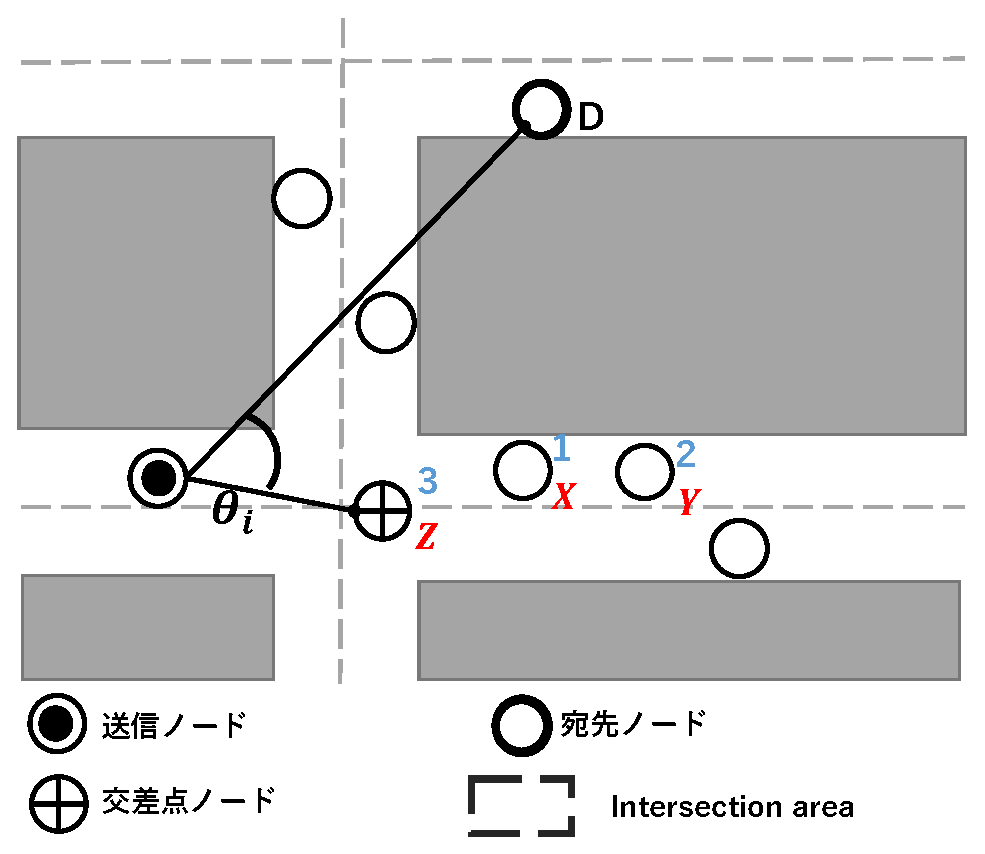
\includegraphics[width=120mm]{figures/aim_SIGO.eps}
	\caption{Local optimum problemが起きやすい優先度}
	\label{fig:aim_SIGO}
\end{figure}




\subsection{優先度スケジューリングアリゴリズム}
\label{SIGO_priority}
SIGOでは, タイマーベースの優先度スケジューリングアルゴリズムを使用する. このアルゴリズムでは, 最も優先度が高いノードが最初にパケットをブロードキャストする. 他の中継候補ノードは, 自身より優先度の高いノードからのパケットを受信すると, 待機中のパケットを破棄する. タイマーが期限切れになり, 自身より優先度の高いノードからのパケットを受信していない場合, RCSの選定, RCSに含まれるノードの優先順位をパケットに含みブロードキャストを開始する. SIGOは, 中継候補ノード$i$の優先度を以下の式\ref{pri-intersection}, \ref{pri}で算出する.

\begin{equation}
	\label{pri-intersection}
	\frac{D_{sd} - D_{id}}{ETX_{i}^{2}} + IRI_i,  D_{id} < D_{sd}
\end{equation}

\begin{equation}
	\label{pri}
	\frac{D_{sd} - D_{id}}{ETX_{i}^{2}} ,   D_{id} < D_{sd}
\end{equation}

ここで, $D_{sd}$は送信ノードから宛先ノードまでの距離, $D_{id}$は各中継候補ノード$i$から宛先ノードまでの距離である. $D_{id}$ \verb|<| $D_{sd}$の条件を満たさない場合は, 優先度の計算は行わずにRCSから除外する. 式\ref{pri-intersection}はノード$i$が交差点ノードの場合, 式\ref{pri}はノード$i$が交差点ノード以外の場合に適用される. また, 式\ref{pri-intersection}, \ref{pri}で算出された値が大きいほどノード$i$の優先度が高くなる.




\section{ORS: Opportunistic Recovery Strategy}
提案したOpportunistic routing(SIGO)は, Local optimum problemに陥ることがある. すなわち, 自分より宛先ノードに近い隣接ノードが存在しない場合である. このLocal optimum problemを解決するために, Recovery strategyが必要である. 本研究では, 従来の中継ノードを一つ選択するユニキャスト型のRecovery strategyとは異なり, SIGOと同様にRCSに向けてパケットをブロードキャストするOpportunistic Recovery strategy(ORS)を提案する. ORSでは, SIGOと同様により高い優先度を持つ中継候補ノードからパケットをブロードキャストする. 自身より優先度の高い中継候補ノードからのパケットを受信した場合, 自身の待機中パケットを破棄する. 提案するORSでは, 中継候補ノードの優先度を決定するメトリックとしてリンク品質とJBRで提案された最小角度法を用いる. 最初にLocal optimum problemに陥ったノードをLSN, LSNにパケットを送信したノード(LSNの1ホップ前のノード)をPLSNとする. LSNは従来のRecovery strategyと同様に, 自身の位置情報をパケットに含めてパケットをブロードキャストする. LSNより宛先に近いノードがパケットを受信した場合, 通常の中継戦略(SIGO)を開始する. また, ORSでは最小角度法を用いるため, Recovery strategyが完了するまで, LSNとPLSNの位置情報が常にパケットに含まれる.
ORSのフローチャートを図\ref{fig:ORS}に示す.

\begin{figure}[!ht]
	\centering
	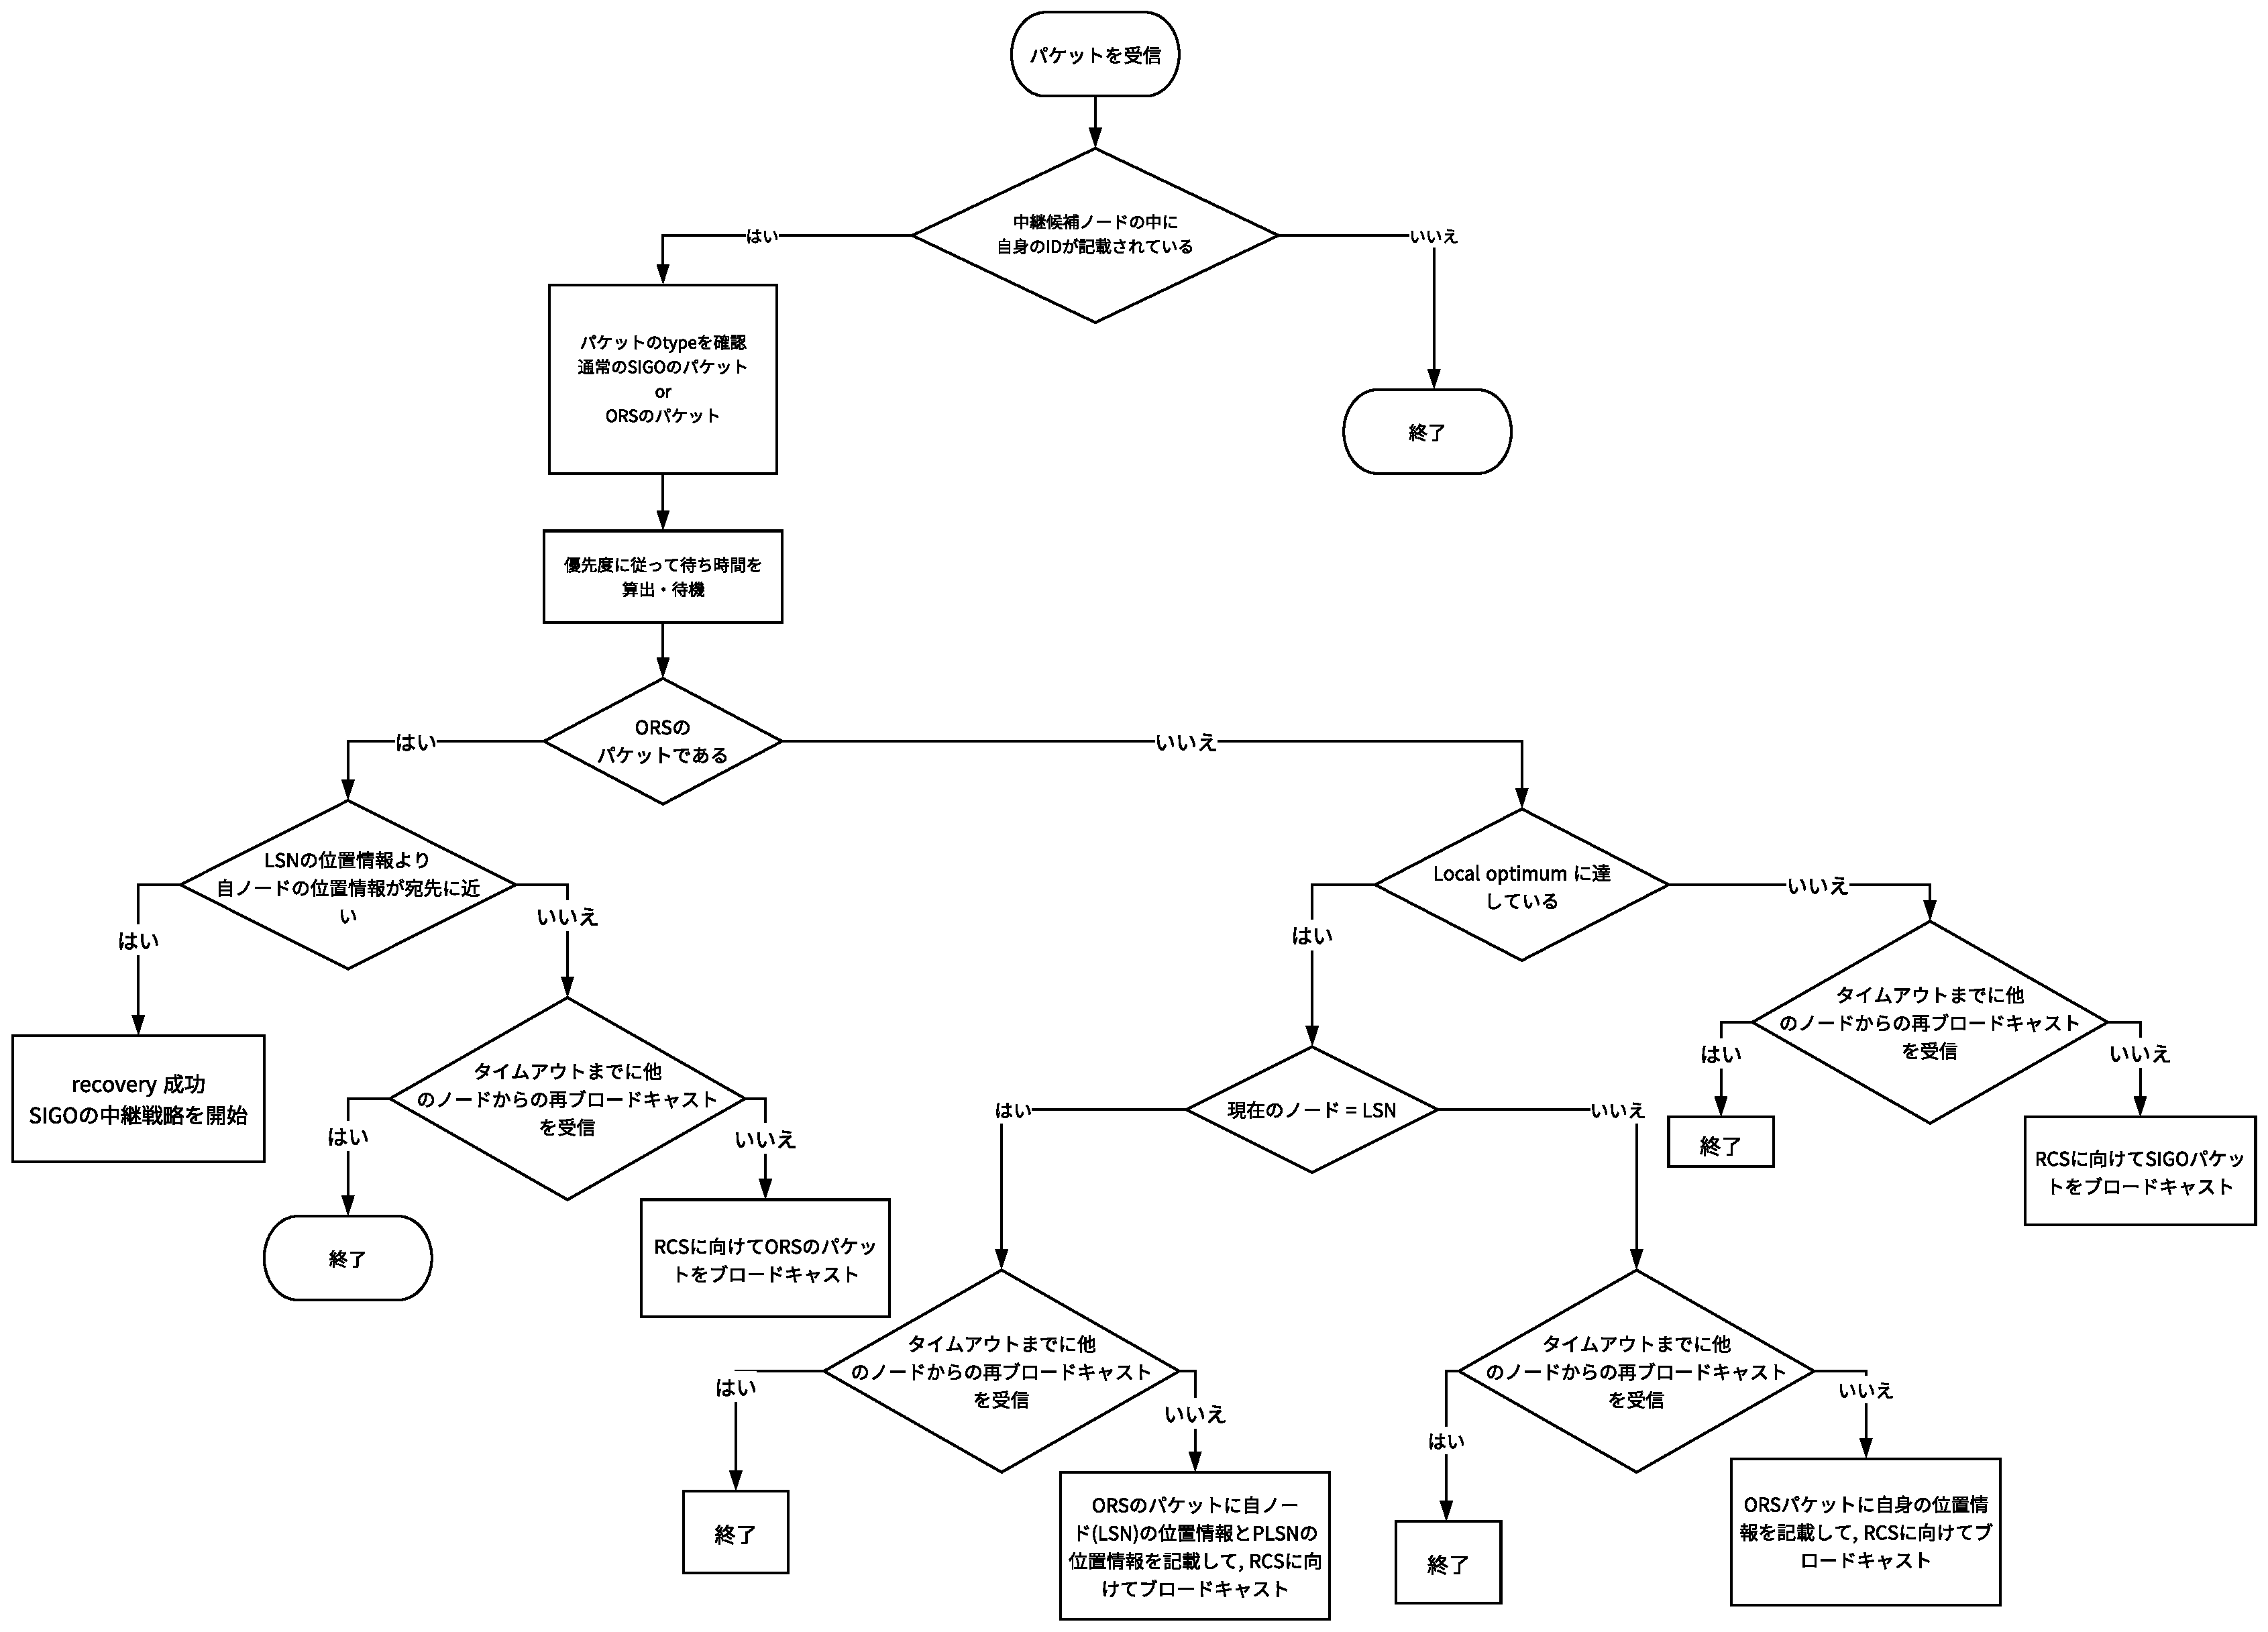
\includegraphics[width=170mm]{figures/ORS.eps}
	\caption{SIGOとORSのフローチャート}
	\label{fig:ORS}
\end{figure}

\subsection{パケットフォーマット}
ORSのデータパケットのフォーマットを図\ref{fig:ORS_packet}に示す.

\begin{itemize}
	\item $SourceId$: ソースノードのID.
	\item $DstId$: 宛先ノードのID.
	\item $Dst_x Pos$: 宛先ノードの$x$座標.
	\item $Dst_y Pos$: 宛先ノードの$y$座標.
	\item $ID_i$: 中継候補ノードの優先度$i$. $i$ = 1, 2, 3, ...(数字が低いほど優先順位が高い) 
	\item $Send_x Pos$: 送信ノードの$x$座標.
	\item $Send_y Pos$: 送信ノードの$y$座標.
	\item $LSN_x Pos$: LSNの$x$座標.
	\item $LSN_y Pos$: LSNの$y$座標.
	\item $PLSN_x Pos$: PLSNの$x$座標.
	\item $PLSN_y Pos$: PLSNの$y$座標.
	\item $Data$: ペイロード部.
\end{itemize}

ここで, $ID_i$, $Send_x Pos$, $Send_y Pos$以外の情報はRecovery strategy中には変更されない. 各Recovery strategyにおける送信ノードは中継候補ノードの優先度情報$ID_i$と自身の位置情報$Send_x Pos$, $Send_y Pos$を更新しブロードキャストする.

\begin{figure}[!ht]
	\centering
	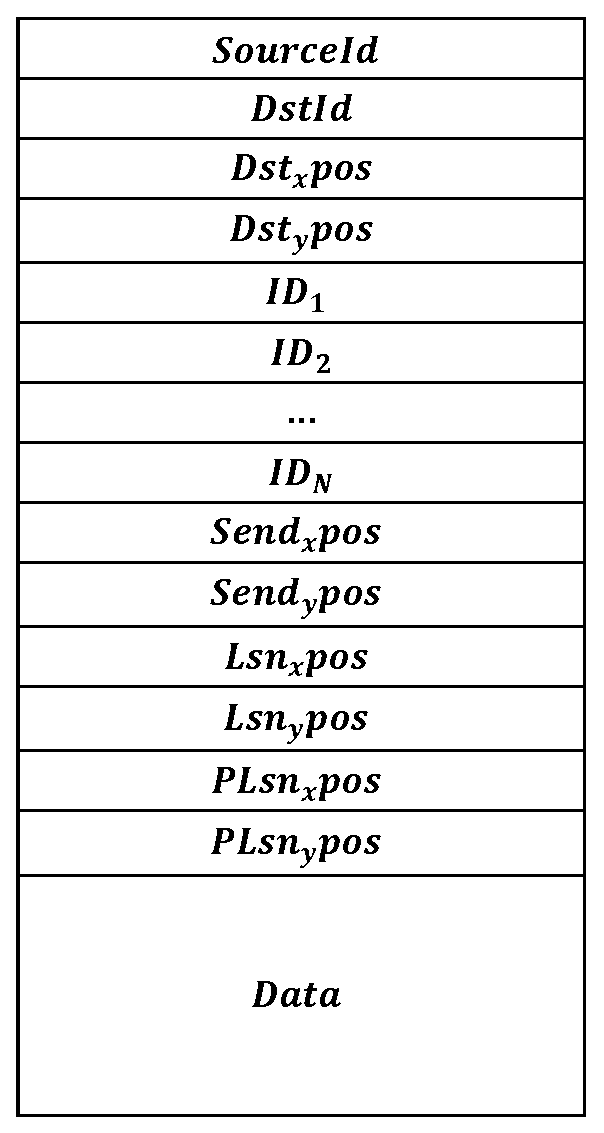
\includegraphics[width=60mm]{figures/ORS_packet.eps}
	\caption{ORSパケットフォーマット}
	\label{fig:ORS_packet}
\end{figure}


\subsection{RCSに含まれるノードの条件}
ORSでは, 条件\ref{potential_nodes}を満たす隣接ノードの中からRCSを選定する. 条件\ref{potential_nodes}を満たさない隣接ノードはRCSの対象外となり後述する優先度の計算も行わない.

\begin{equation}
	\label{potential_nodes}
	\left( nldis_i > cldis \right)   AND   \left( nldis_i > mndis_i \right) 
\end{equation}

$cldis$は送信ノードと送信ノードの1ホップ前のノード(送信ノードにパケットを送信したノード)との距離, $nldis$は送信ノードの1ホップ前のノードと検討中のノード(RCSに含まれる条件を満たすノード)の距離, $mndis$は送信ノードと検討中のノードの距離である(図\ref{fig:Condition_RCS}). 

\begin{figure}[!ht]
	\centering
	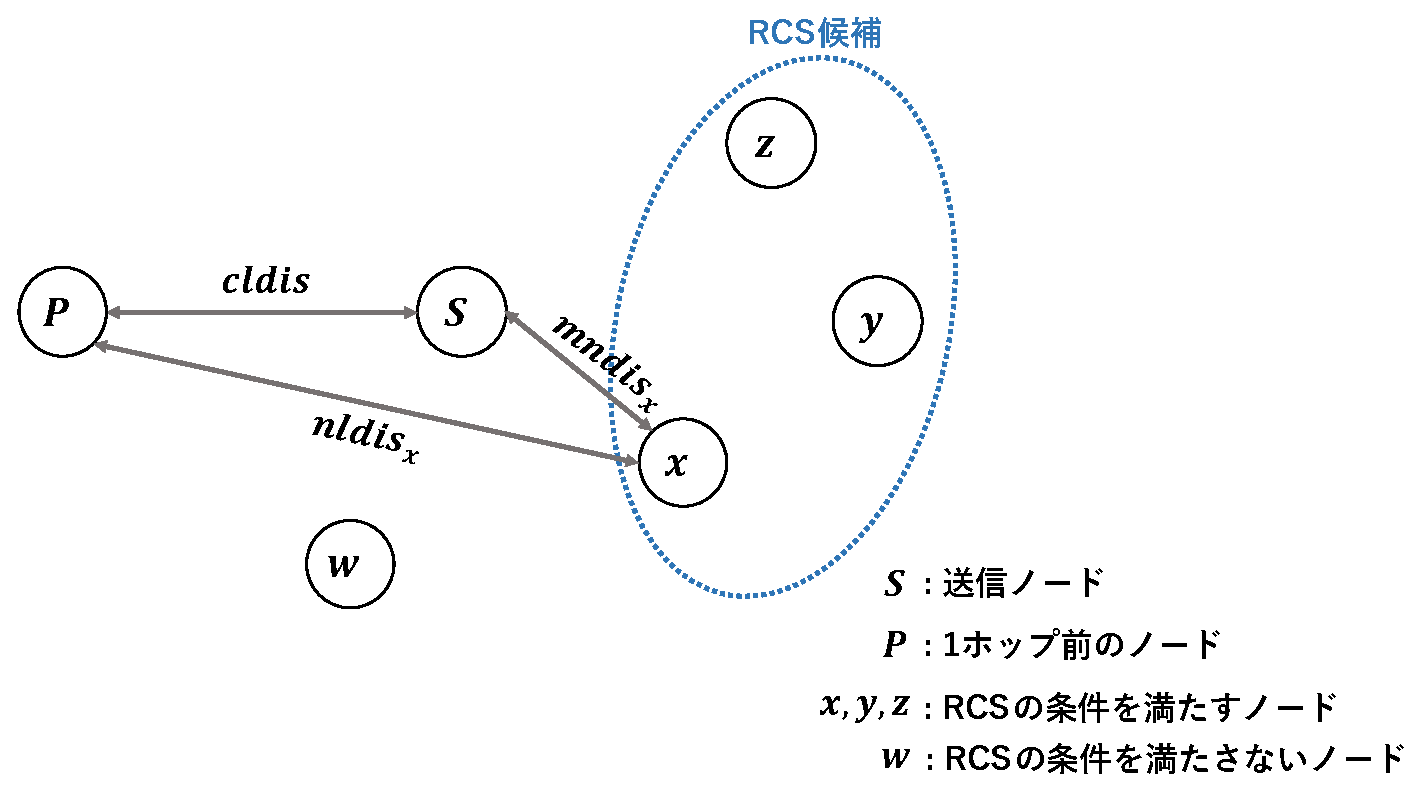
\includegraphics[width=150mm]{figures/Condition_RCS.eps}
	\caption{RCSに含まれるノードの条件}
	\label{fig:Condition_RCS}
\end{figure}


\subsection{最小角度法}
ORSでは, 中継候補ノードの優先度を決定するメトリックの1つとして最小角度法を用いる. ORSにおける各送信ノード(LSNも含む)は, 条件\ref{potential_nodes}を満たす各隣接ノード$i$の$sdangle$と$snagle_i$を算出する(図\ref{fig:minangle}).
$sdangle$はLSNと宛先ノードを結ぶ直線とLSNとPLSNを結ぶ直線のなす角度である. $snangle_i$はLSNとRCSの条件を満たす中継候補ノード$i$を結ぶ直線とLSNとPLSNを結ぶ直線のなす角度である. 
次に算出した$snangle$と$sdangle$を用いて, 式\ref{minangle}で中継候補ノード$i$の$minangle_i$を算出する.

\begin{equation}
	\label{minangle}
	minangle_i = \mid sdangle - snangle_i \mid
\end{equation}

\begin{figure}[!ht]
	\centering
	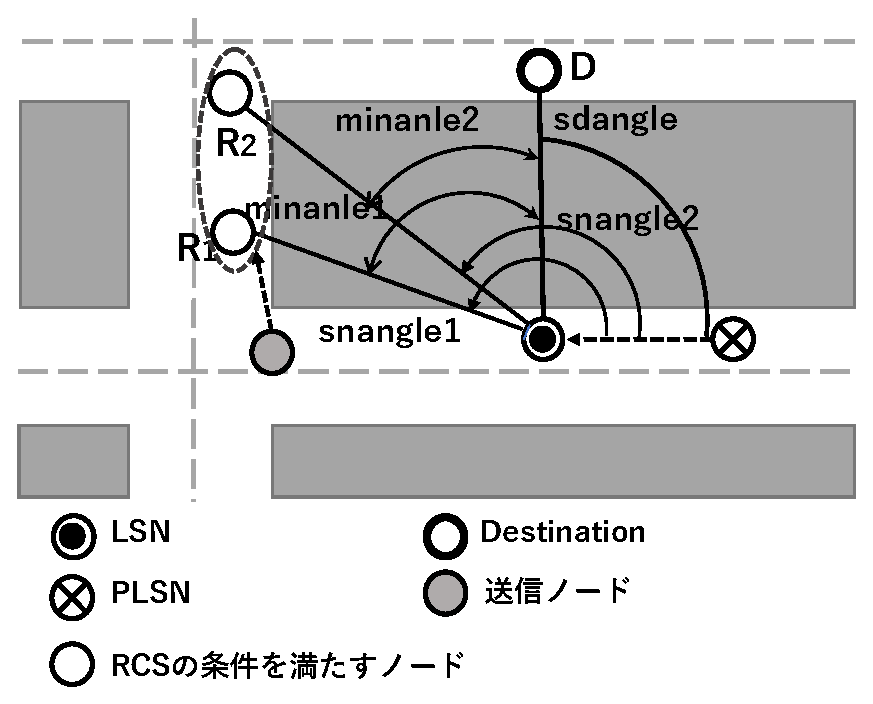
\includegraphics[width=130mm]{figures/minangle.eps}
	\caption{最小角度法}
	\label{fig:minangle}
\end{figure}


\subsection{優先度スケジューリングアリゴリズム}
\label{ORS_priority}

ORSでは, SIGOと同様にタイマーベースの優先度スケジューリングアルゴリズムを使用する. ORSにおいて, 各送信ノードは中継候補ノード$i$の優先度を式\ref{sameORS}, \ref{diffORS}で算出する. 

\begin{equation}
	\label{sameORS}
	\frac{360 - minangle_i}{ETX_{i}^{2}} + mndis_i
\end{equation}

\begin{equation}
	\label{diffORS}
	\frac{360 - minangle_i}{ETX_{i}^{2}} 
\end{equation}

ここで, 式\ref{sameORS}は, 送信ノードと中継候補ノード$i$が同一道路セグメントに存在する場合, または中継候補ノード$i$が交差点ノードの場合に適応される. それ以外の場合は, 式\ref{diffORS}が適応される.
また, 式\ref{sameORS}, \ref{diffORS}で算出された値が大きいほどノード$i$の優先度が高くなる.
式\ref{sameORS}において, $mndis_i$を加算する理由は, 図\ref{fig:aim_minangle}のように, 送信ノード$N_1$によって交差点ノードもしくは交差点に近いノードを中継候補ノードとして選択されやすくするためである. この図の場合, リンク品質が同じ場合は高確率で$N_4$が最も優先度が高くなる. $N_4$などの交差点に近いノードが次に中継を開始すると図の$A$や$B$などの$minangle$が小さいノードが選択され, Recoveryの成功率(LSNより宛先に近いノードにパケットが到達する確率) が高くなる. 



\begin{figure}[!ht]
	\centering
	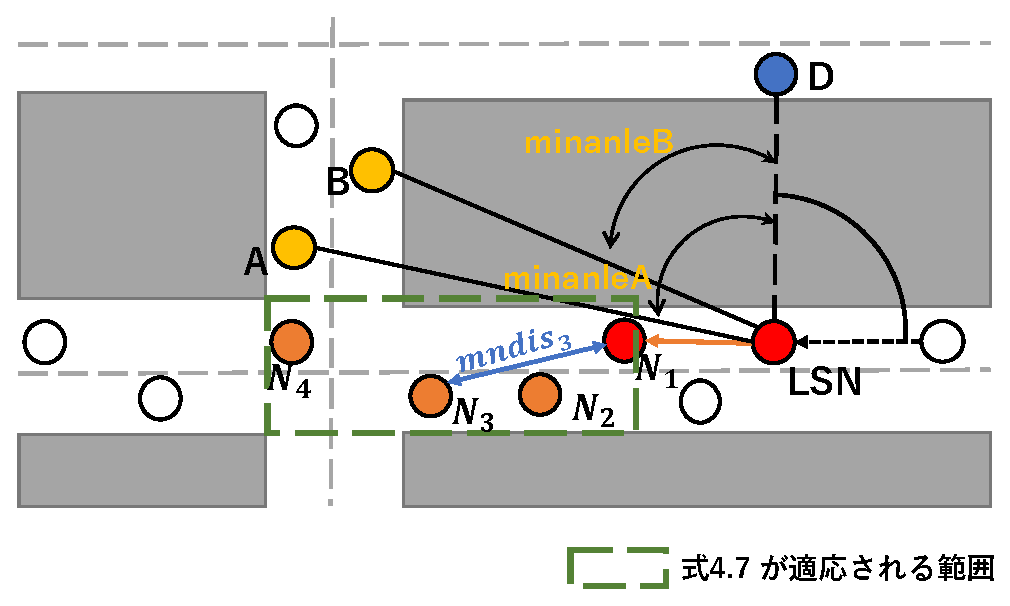
\includegraphics[width=130mm]{figures/aim_minangle.eps}
	\caption{式\ref{sameORS}の目的}
	\label{fig:aim_minangle}
\end{figure}


\section{Geocast routingへの拡張}
本研究では, \ref{SIGO}節のSIGOをGeocastに拡張した転送手法(GSIGO)を提案し, SIGOがGeocast routingにおいても有効であることを示す. GSIGOでは, 主に2種類転送方法に分類できる(図\ref{fig:Geocast}). 1つ目は, Geocast regionの中心座標(SIGOにおける宛先ノードの位置情報)を目指したSIGOと同様の転送手法. 2つ目は, Geocast region内に存在するノード全体にパケットを拡散するためのフラッディングである. したがって, Geocast Regionに到達するまでは1つめの転送方式であるSIGO, Geocast Regionに到達すると2つめの転送手法であるフラッディングに切り替わる. 
GSIGOでは, ソースノードはGeocast regionに関する情報とRCSとして選択したノードの優先度情報をパケットに含みブロードキャストを行う.
パケットを受信した各ノードは, geocast regionに存在するか否かで動作が異なる.

\par
\vspace{5mm}
\noindent
\textbf{Geocast regionに存在しない場合}
\vspace{5mm}

各受信ノードは, パケットに自身のIDが含まれている場合, SIGOの優先度スケジューリングアルゴリズムに従う. それ以外はパケットを破棄する. また, フラッディングによるパケットを受信した場合, 受信したパケットを送信したノードがGeocast regionに存在する場合のみ, フラッディングを行う. これはソースノードがデータパケット生成時に, Geocast Regionに存在したノードがデータパケットを転送中にGeocast Regionの外に移動してしまう可能性があるため, それらのノードにもパケットを届けるために行う. 受信したパケットを送信したノードがGeocast regionに存在しない場合は, パケットを破棄する.

\par
\vspace{5mm}
\noindent
\textbf{Geocast regionに存在する場合}
\vspace{5mm}

各受信ノードはパケットを受信した場合, フラッディングを行う. 

\par
また, Geocast regionに存在するか否かに関係なく, 過去に一度受信したことがあるパケットを受信した場合は, パケットを破棄する.
GSIGOのフローチャートを図\ref{fig:Geocast_flowchart}に示す.



\begin{figure}[!ht]
	\centering
	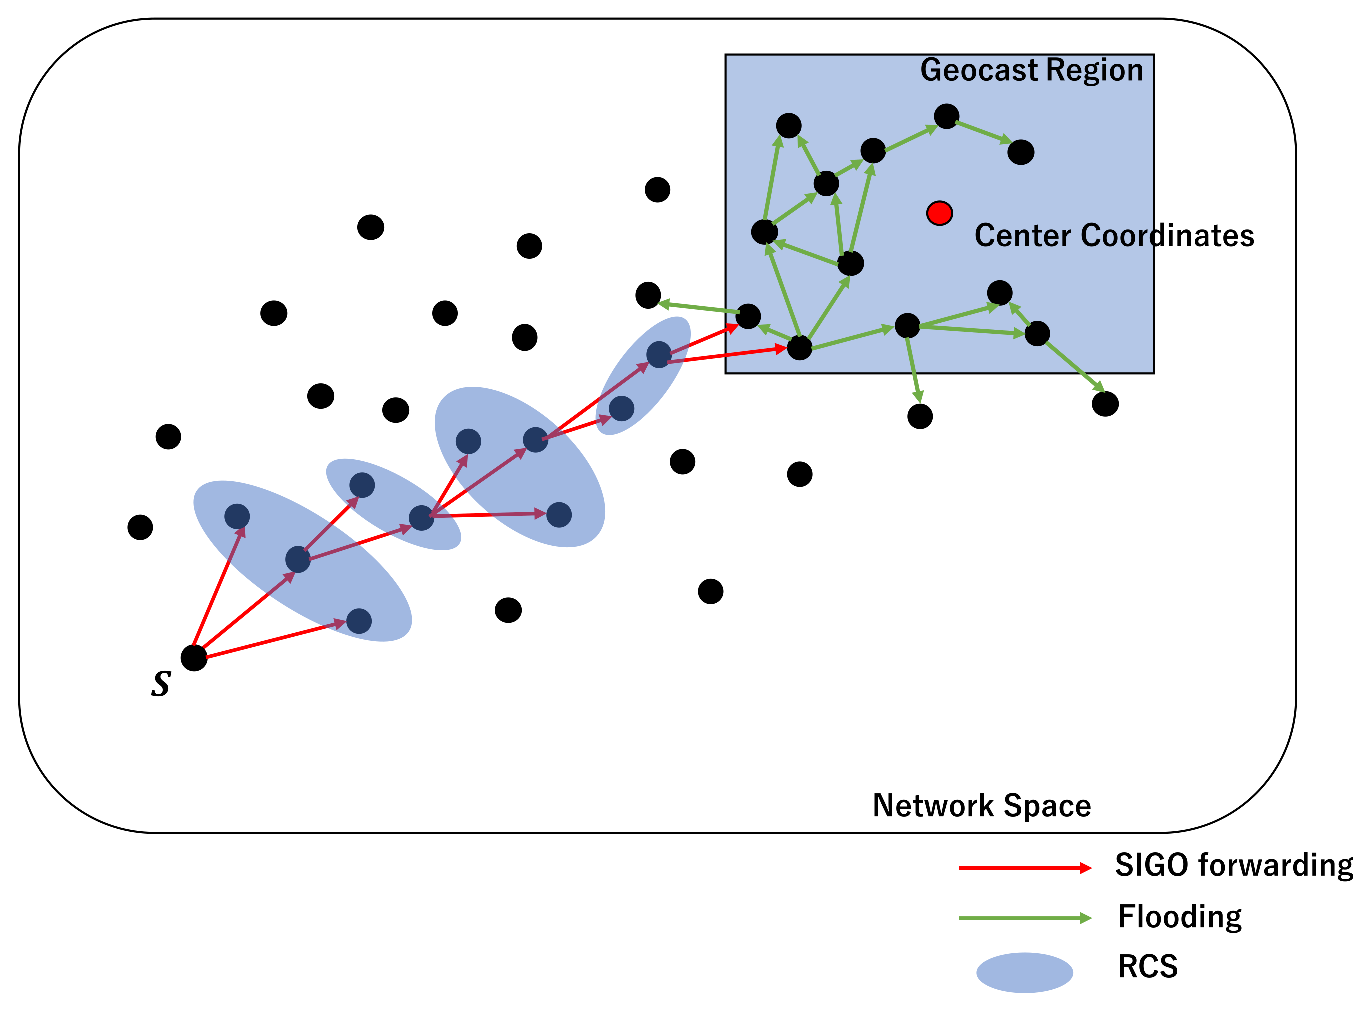
\includegraphics[width=130mm]{figures/Geocast.eps}
	\caption{GSIGOの概要}
	\label{fig:Geocast}
\end{figure}

\begin{figure}[!ht]
	\centering
	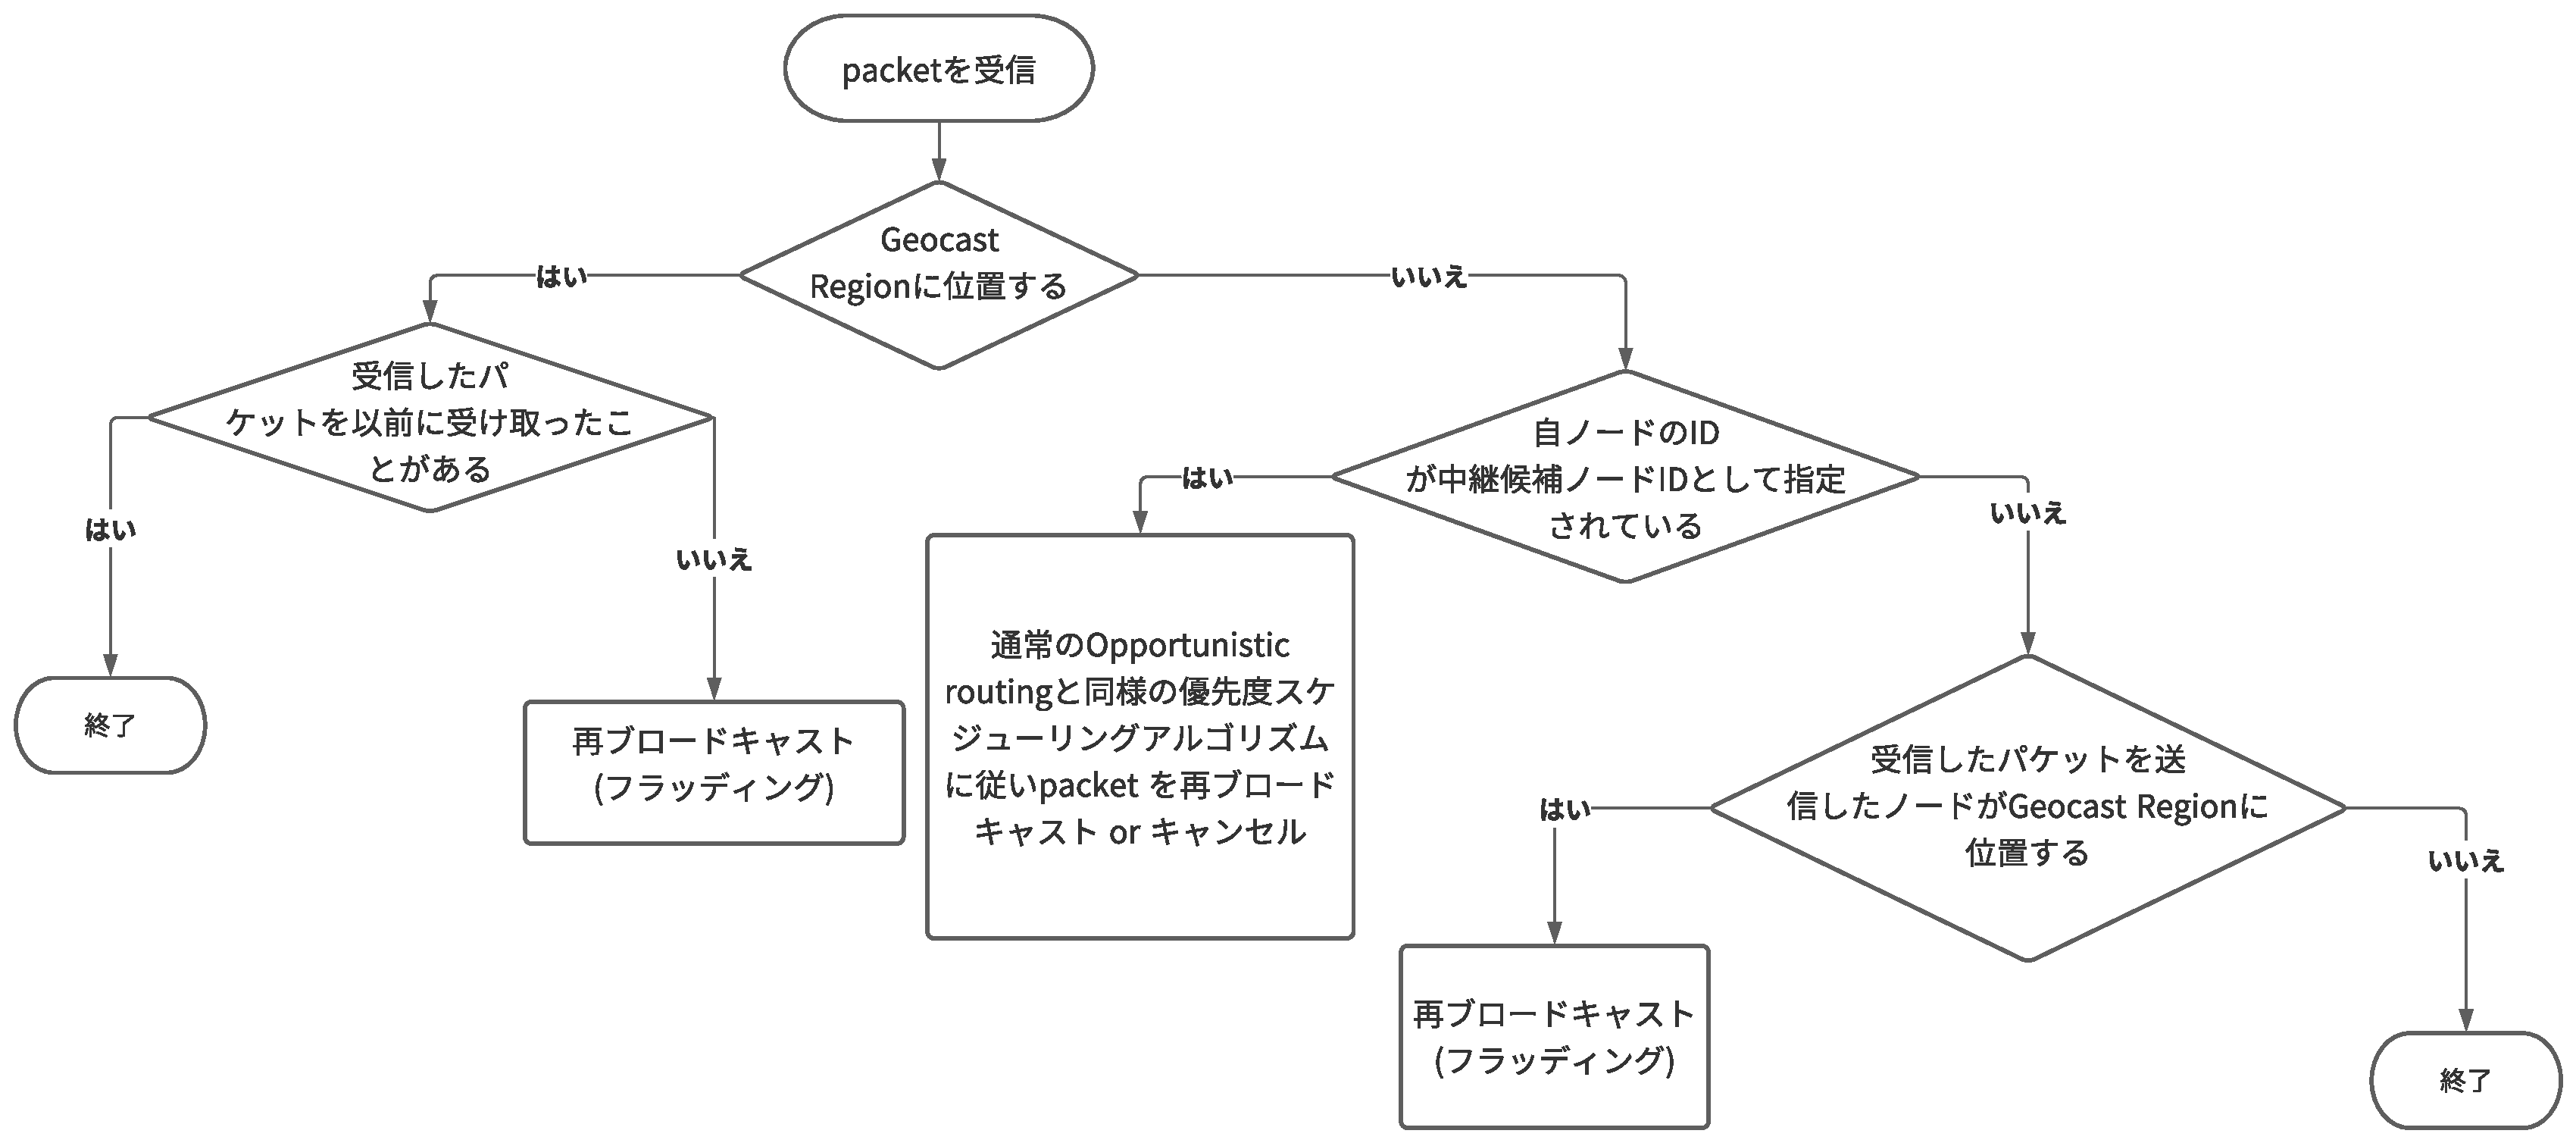
\includegraphics[width=150mm]{figures/Geocast_flowchart.eps}
	\caption{GSIGOフローチャート}
	\label{fig:Geocast_flowchart}
\end{figure}


\chapter{性能評価}
\label{Evaluation}
\section{概要}
本シミュレーションでは, 提案した3つのプロトコル(SIGO, ORS, GSIGO)を\ref{LSGO_evaluation}節と同様のシミュレーション設定とシミュレーションシナリオで評価した. また, 各プロトコル共にRCS数の最大値は5に設定した. したがって各送信ノードは, 隣接ノードの優先順位を計算し, 優先度が高い順に5つのノードをRCSに選定する. また, シャドウイングの強度による通信性能の影響を調査するため, 式\ref{shadowing}のシャドウイングパラメータ$\alpha$(値が大きいほどシャドウイングの強度が増加する)を変化させて評価を行った. 


\section{Opportunistic routingの評価}
\label{SIGO_evaluation}
本節では, SIGOの有効性を評価するため, PDR, エンドツーエンド遅延, オーバーヘッドの3つの評価項目を用いてLSGOと比較した.
各評価項目の算出方法は\ref{evaluation_item}節と同様である. また, ORSの有効性を評価するためJBRと比較した. 以下のシミュレーション結果のグラフにおいて, SIGOはRecovery strategyなしの結果, SIGO + ORSはSIGOのRecovery strategyとしてORSを用いたときの結果, SIGO + JBRはRecovery strategyとしてJBRを用いたときの結果を表す. 

%\par
%\vspace{5mm}
%\noindent
%\textbf{パケット到達率(PDR) : ノード数変化}
%\vspace{5mm}
\subsection{パケット到達率 (PDR) : ノード数変化}

図\ref{fig:SIGO_PDR_num}は, シャドウイングパラメータを変化させたときのPDRを示している.
図に示す通り, PDRの評価では以下の結果が得られた.
(1) ノード数が増加するほど, すべてのプロトコルのPDRが増加する. 
(2) ノード数が増加するほど, SIGOとLSGOの差が大きくなり, 通信性能の向上を果たしている.
(3) ノード数に関係なく, ORSはSIGOよりPDRが増加しているので, recoveryに成功(LSNより宛先に近いノードにパケットが転送された)しているといえる. 一方で, JBRはORSと比較すると, recoveryの成功率が低い. 
(1)の結果はノード数が増加するほど, 各送信ノードの隣接ノード数が増加し, RCS数が増加することが原因だと推測される.
(2)の結果はシャドウイングパラメータが増加するほど, LSGOは 図\ref{fig:LSGO-problem}(a)のようにLocal optimum problemに陥る可能性が高まるのに対して, SIGOでは交差点ノードを優先することで図\ref{fig:LSGO-problem}(b)のようにこの問題をを回避していることが原因だと推測される (Opportunistic routingの評価ではrecovery stratyは未実装であるため, Local optimum problemに陥るとパケットをドロップする). また, ノード数が増加するほど, 送信ノードの隣接ノードに交差点ノードが存在する確率が増加するためだと推測できる.
(3) の結果は, JBRは中継ノードを1つに決定することと, リンク品質を考慮していないため, ORSと比較してLSNより宛先に近いノードにパケットが到達するまでにパケットロスが発生したと推測される. 

\begin{figure}[!ht]
	\centering
	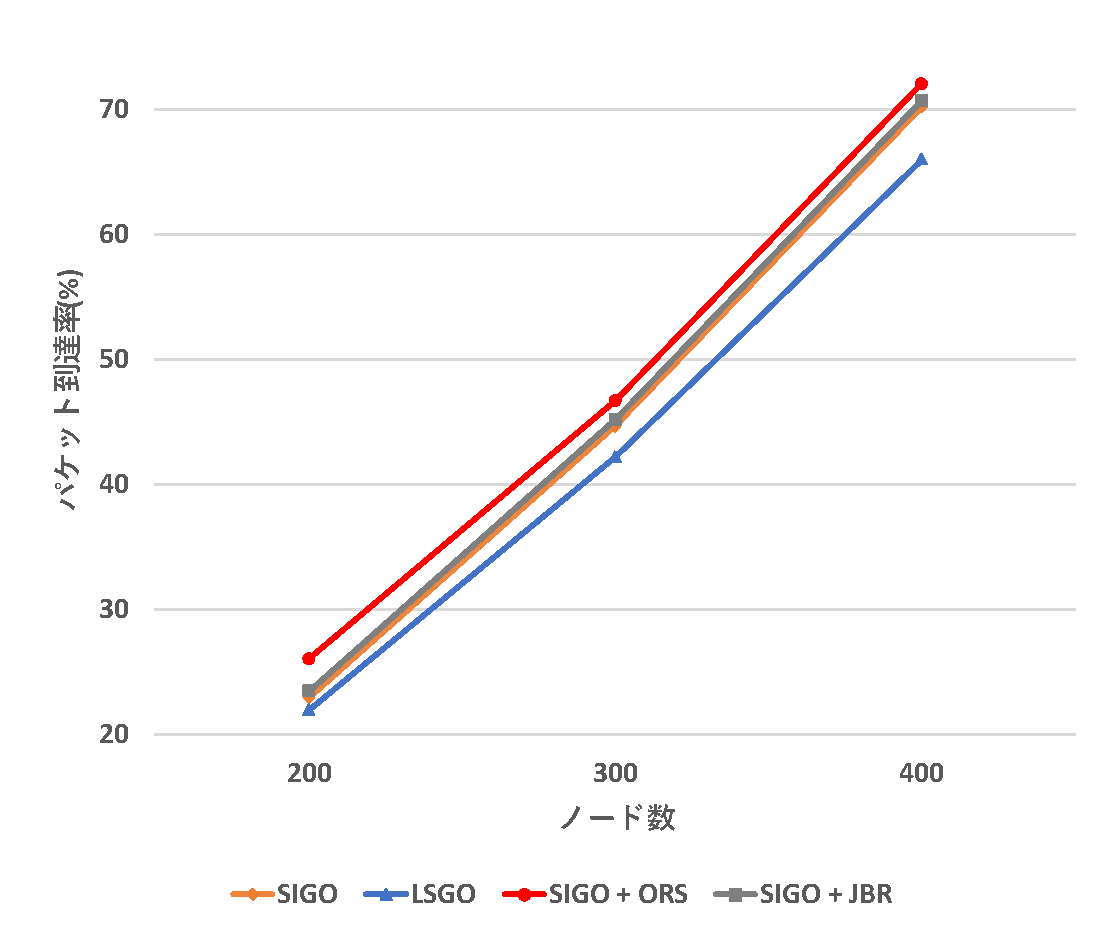
\includegraphics[width=110mm]{figures/SIGO_PDR_num.eps}
	\caption{パケット到達率 vs ノード数}
	\label{fig:SIGO_PDR_num}
\end{figure}

\subsection{エンドツーエンド遅延 : ノード数変化}
図\ref{fig:SIGO_delay_num}は, ノード数を変化させたときのエンドツーエンド遅延を示している.
図に示す通り, エンドツーエンド遅延の評価では以下の結果が得られた.
(1) ノード数が増加するほど, すべてのプロトコルのエンドツーエンド遅延が増加する.
(2) 提案プロトコル (SIGO, ORS)の遅延に対する影響は非常に小さいものである. 
(3) SIGO + JBRの遅延が他のプロトコルと比較して少ない. 
Opportunistic routingにおいて, 遅延に最も影響を与えるのは, より優先度の高い中継候補ノードにパケットが到達するかどうかである. 例えば, 優先度1のパケットが受信すると中継タイマーが0秒で再ブロードキャストされるのに対して, 2, 3, 4, 5と優先度が低い中継候補ノードのみパケットを受信した場合, 優先度に応じて待ち時間が発生する.
そして, (1)の結果はノード数が増加するほど各送信ノードが選択するRCS数が増加するため, より優先度の高い中継候補ノードにパケットが到達しなかった場合遅延が増加したと推測される. 
(2)の結果は, 本研究で提案したSIGO, ORSはLSGOとリンク品質の算出を同様の方法で行うため, より優先度の高い中継候補ノードにパケットが到達する確率はほとんど差が生じないので, 遅延の差が小さかったと推測される. 
(3)の結果はJBRは中継ノードを1つに選択し, 中継タイマーを用いずにパケットを再転送するため遅延が小さかったと推測される. 

\begin{figure}[!ht]
	\centering
	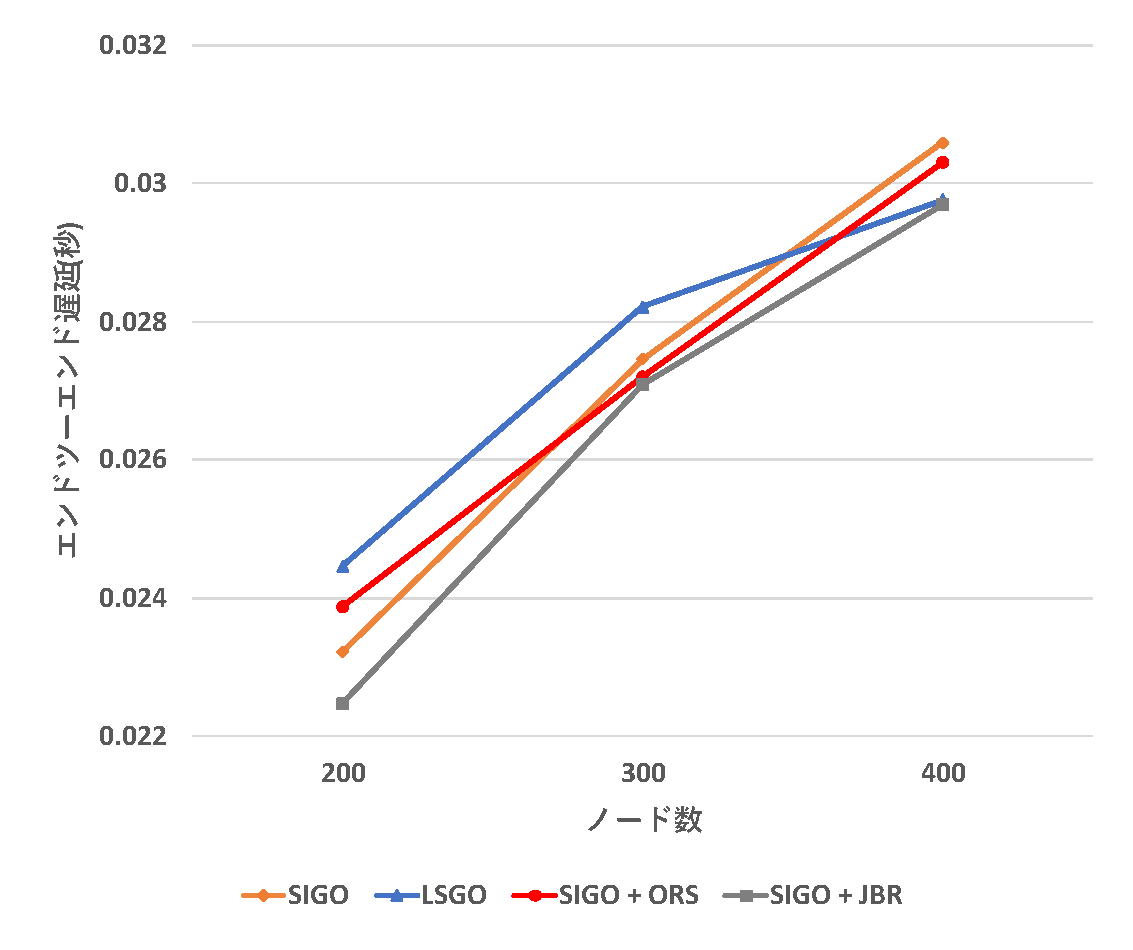
\includegraphics[width=110mm]{figures/SIGO_delay_num.eps}
	\caption{エンドツーエンド遅延 vs ノード数}
	\label{fig:SIGO_delay_num}
\end{figure}

\subsection{オーバーヘッド : ノード数変化}

図\ref{fig:SIGO_overhead}は, ノード数を変化させたときのオーバーヘッドを示している.
図に示す通り, 以下の3つの結果が得られた.
(1) ノード数が増加するほど, すべてのプロトコルのオーバーヘッドが減少する.
(2) ノード数に関係なく, SIGOとLSGOの差は小さい. 
(3) ORS, JBRともにSIGOと比較してオーバーヘッドが増加している. 
(1)の結果は, すべてのプロトコルにおいてノード数が増加すると, 各送信ノードに隣接するノード数が増加し, 宛先ノードが正常にパケットを受信した総数が増加するからだと推測される.
(2)の結果は, SIGOはLSGOと比較してパケット到達率が上昇しているにもかかわらず, オーバーヘッドの差が小さいため, パケット数を増加させずに宛先ノードまで正常にパケットが到達していることを示している. 
(3)の結果は, 通常の中継戦略(SIGO, LSGO)はパケットを送信するたびに, パケットが宛先ノードの方向へ中継されるのに対して, recovery strategy(ORS, JBR)では宛先ノードから遠ざかる方向へ中継される可能性があるからである.
図\ref{fig:Recocvery_overhead_reason}にこの状況の一例を示す.

\begin{figure}[!ht]
	\centering
	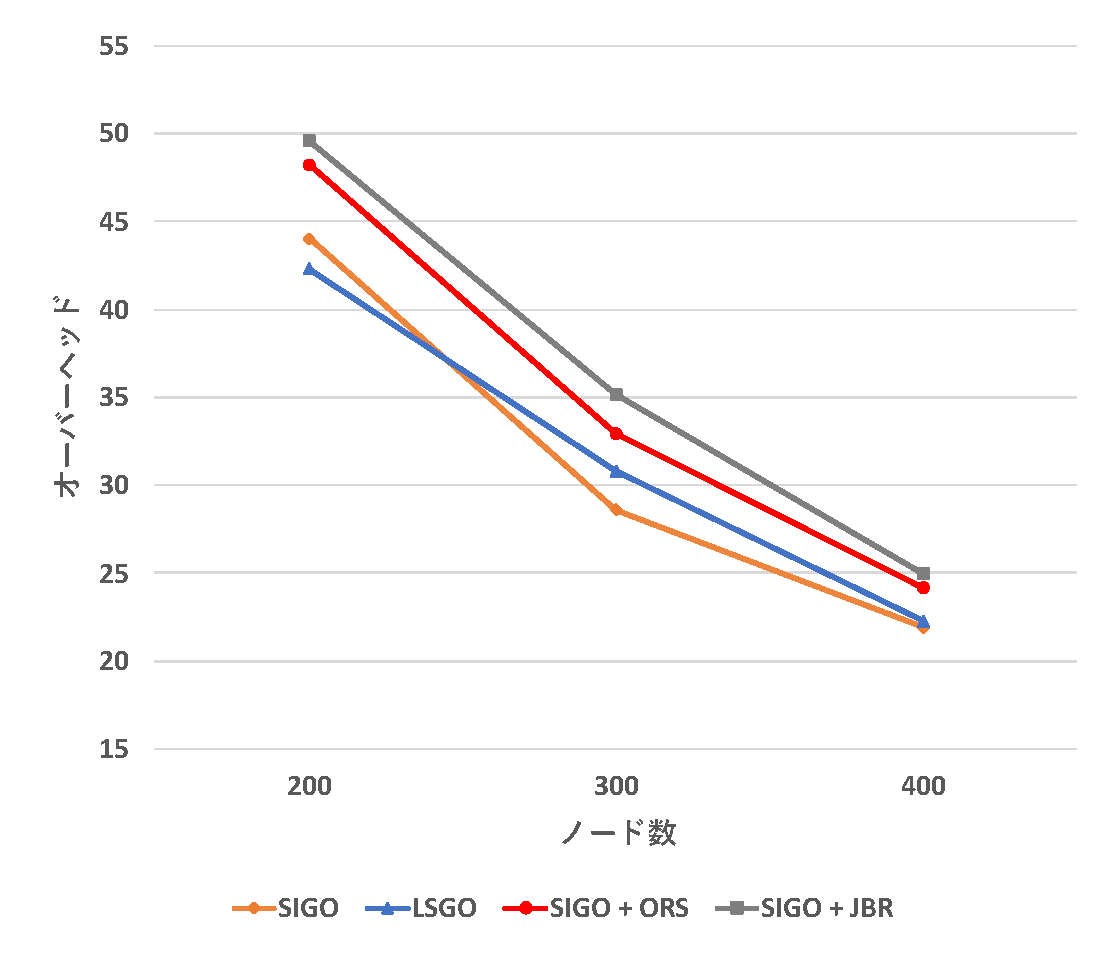
\includegraphics[width=110mm]{figures/SIGO_overhead_num.eps}
	\caption{オーバーヘッド vs ノード数}
	\label{fig:SIGO_overhead}
\end{figure}

\begin{figure}[!ht]
	\centering
	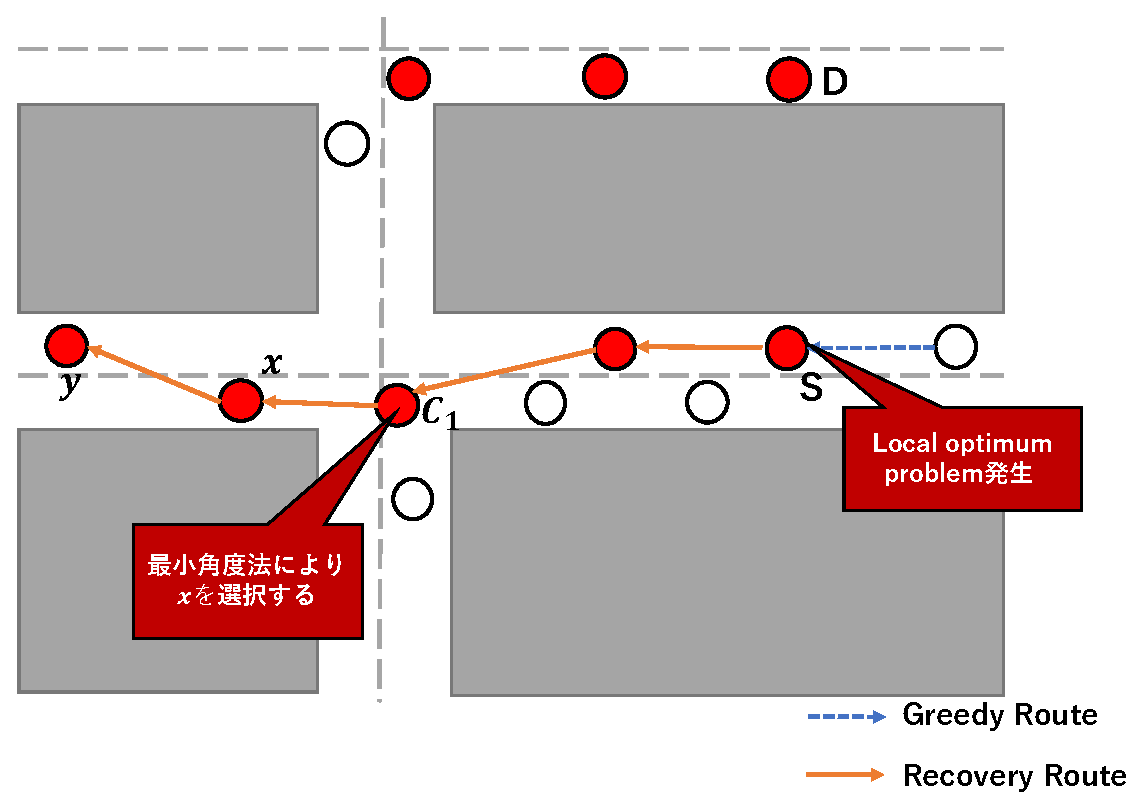
\includegraphics[width=120mm]{figures/Recovery_overhead_reason.eps}
	\caption{Recovery Strategyにおいてオーバーヘッドが増加する原因}
	\label{fig:Recocvery_overhead_reason}
\end{figure}


\subsection{パケット到達率 (PDR) : シャドウイング強度変化}
図\ref{fig:SIGO_PDR_shadow}は, ノード数を変化させたときのPDRを示している.
図に示す通り, PDRの評価では以下の結果が得られた.
(1) シャドウイングパラメータが増加するほど, すべてのプロトコルのパケット到達率が減少する.
(2) シャドウイングパラメータが増加するほど, SIGOはLSGOと比較してパケット到達率が上昇する.
(3) シャドウイングパラメータに関係なく, ORSはSIGOよりPDRが増加しているので, recoveryに成功(LSNより宛先に近いノードにパケットが転送された)しているといえる. 一方で, JBRはORSと比較すると, recoveryの成功率が低い.
(1) の結果はシャドウイングの影響で送信ノードの隣接ノード数が減少し, RCSにパケットが届きにくくなったこと原因だと推測される. 
(2) の結果は, 図\ref{fig:LSGO-problem}のようにシャドウイングパラメータが増加するほどLSGOではLocal optimum problemに陥る確率が高まるのに対して, SIGOでは交差点ノードを中継候補ノードとして選択されやすくすることでこれを回避していることが原因だと推測される. 
(3) JBRは中継ノードを1つに決定することと, リンク品質を考慮していないため, ORSと比較してLSNより宛先に近いノードにパケットが到達するまでにパケットロスが発生したと推測される. 


\begin{figure}[!ht]
	\centering
	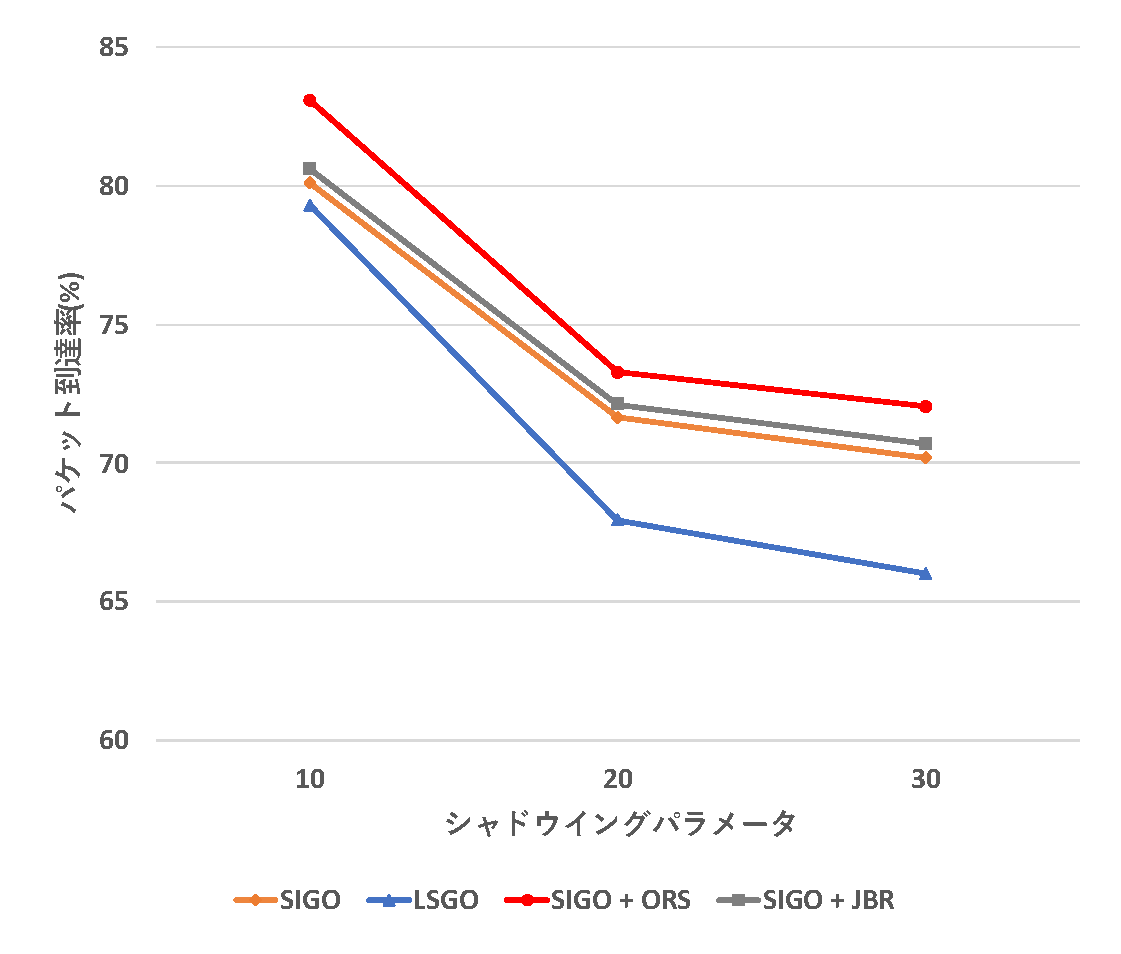
\includegraphics[width=120mm]{figures/SIGO_PDR_shadow.eps}
	\caption{パケット到達率 vs シャドウイング強度}
	\label{fig:SIGO_PDR_shadow}
\end{figure}

\subsection{エンドツーエンド遅延 : シャドウイング強度変化}
図\ref{fig:SIGO_delay_shadow}は, ノード数を変化させたときのPDRを示している.
図に示す通り, PDRの評価では以下の結果が得られた.
(1) シャドウイングパラメータが増加するほど, すべてのプロトコルの遅延が増加する.
(2) LSGOと比較して, シャドウイングパラメータが増加するほど, SIGOの遅延が増加する.
(3) シャドウイングパラメータに関係なく, ORSはJBRと比較して遅延が大きい. 
(1)の結果は, シャドウイングパラメータが増加するほど建物による電波減衰が起こり, 建物を通過するパケットが届きにくくなることで,  ソースノードと宛先ノードを直線的に結ぶような経路が形成することが難しくなったことが原因だと推測される.
(2) の結果は, SIGOではシャドウイングの強度が強くなるほど, 式\ref{pri-intersection}のIRIが増加し, リンク品質(ETX)が悪い場合でも優先度が高くなるため, 交差点ノードにパケットが届かなかった場合に遅延が増加したと推測される.
(3) の結果はJBRは中継ノードを1つに選択し, 中継タイマーを用いずにパケットを再転送するため遅延が小さかったと推測される.


\begin{figure}[!ht]
	\centering
	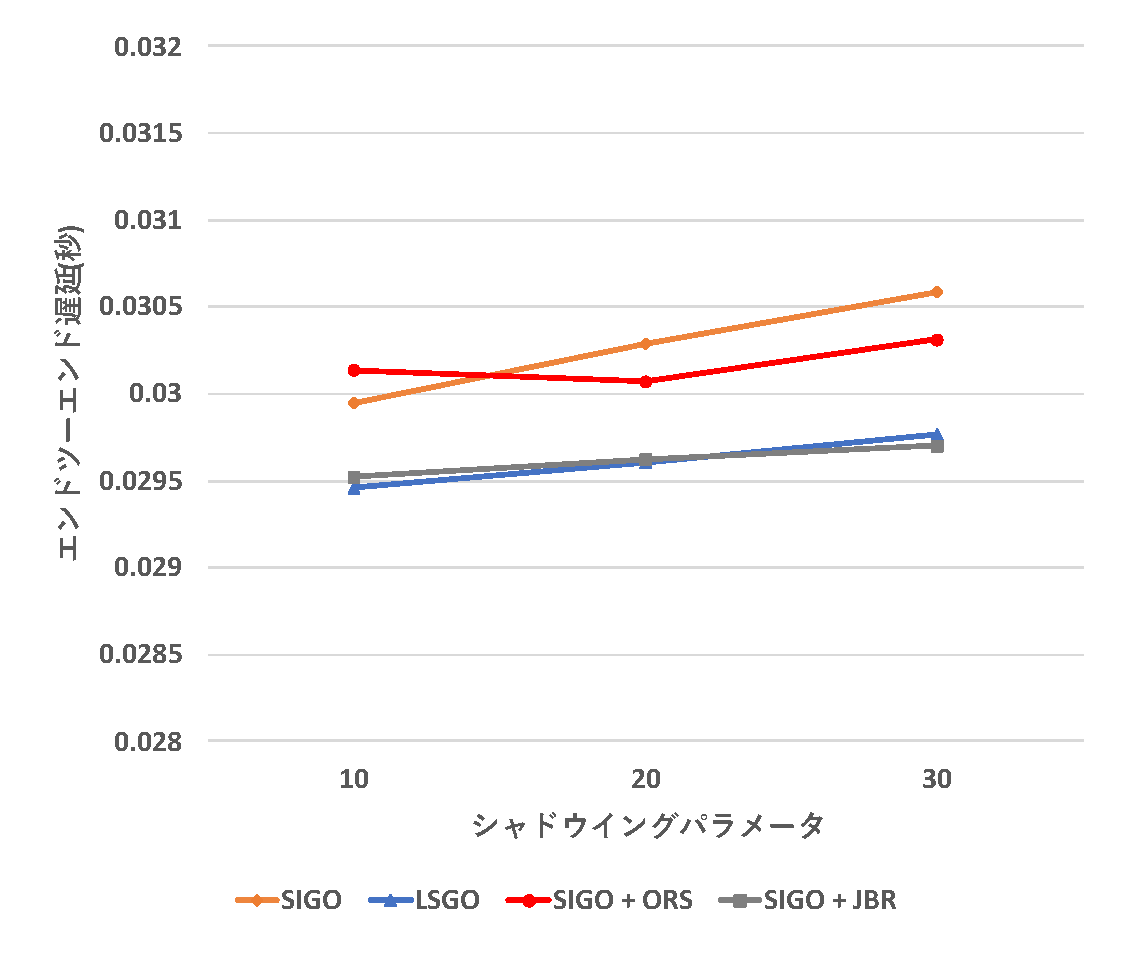
\includegraphics[width=120mm]{figures/SIGO_delay_shadow.eps}
	\caption{エンドツーエンド遅延 vs シャドウイング強度}
	\label{fig:SIGO_delay_shadow}
\end{figure}


\subsection{オーバーヘッド : シャドウイング強度変化}
図\ref{fig:SIGO_overhead_shadow}は, ノード数を変化させたときのオーバーヘッドを示している.
図に示す通り, オーバーヘッドの評価では以下の結果が得られた.
(1) シャドウイングパラメータが増加するほど, すべてのプロトコルのオーバーヘッドが増加する.
(2) SIGO + ORSはSIGOと比較してシャドウイングパラメータが増加するほど, オーバーヘッドが増加する.
(3) シャドウイングパラメータに関係なく, JBRのオーバーヘッドは他のプロトコルと比較して増加している.
(1) の結果は, シャドウイングパラメータが増加するほど宛先ノードが正常にパケットを受信した総数が減少することと, RCSを異なるroad segmentに存在するノードから選定した場合, シャドウイングパラメータが増加するほど再ブロードキャストキャンセルが行われない可能性が高まるからである. 図\ref{fig:dif_roadsegment_overhead_reason}にこの状況の一例を示す.
この例ではノード$S$が図のように優先度を決定しパケットをブロードキャストする. 受信した中継候補ノードは自身の優先順位に従ってパケットを再ブロードキャストする. この場合では優先度1のノードが最初に再ブロードキャストを行っている. しかしこの場合, 優先度2, 3のノードは優先度1からのパケットをシャドウイングの影響で受信できない場合がある. このような状況では優先度2, 3のノードの再ブロードキャストがキャンセルされないため, 冗長なパケットが増加する. その結果としてオーバーヘッドが増加したと推測される.
(2) の結果は, シャドウイングパラメータが増加するほど図\ref{fig:Recocvery_overhead_reason}のように宛先ノードから遠ざかるルートが形成される可能性が高まるからである. 
(3) の結果は, JBRはORSと比較して宛先ノードから遠ざかるルートが形成される可能性が高いことに加え, recoveryの成功率が低く, 宛先ノードが正常にパケットを受信する数がSIGOに比べて増加していないので, 結果としてオーバーヘッドが増加したと推測される.


\begin{figure}[!ht]
	\centering
	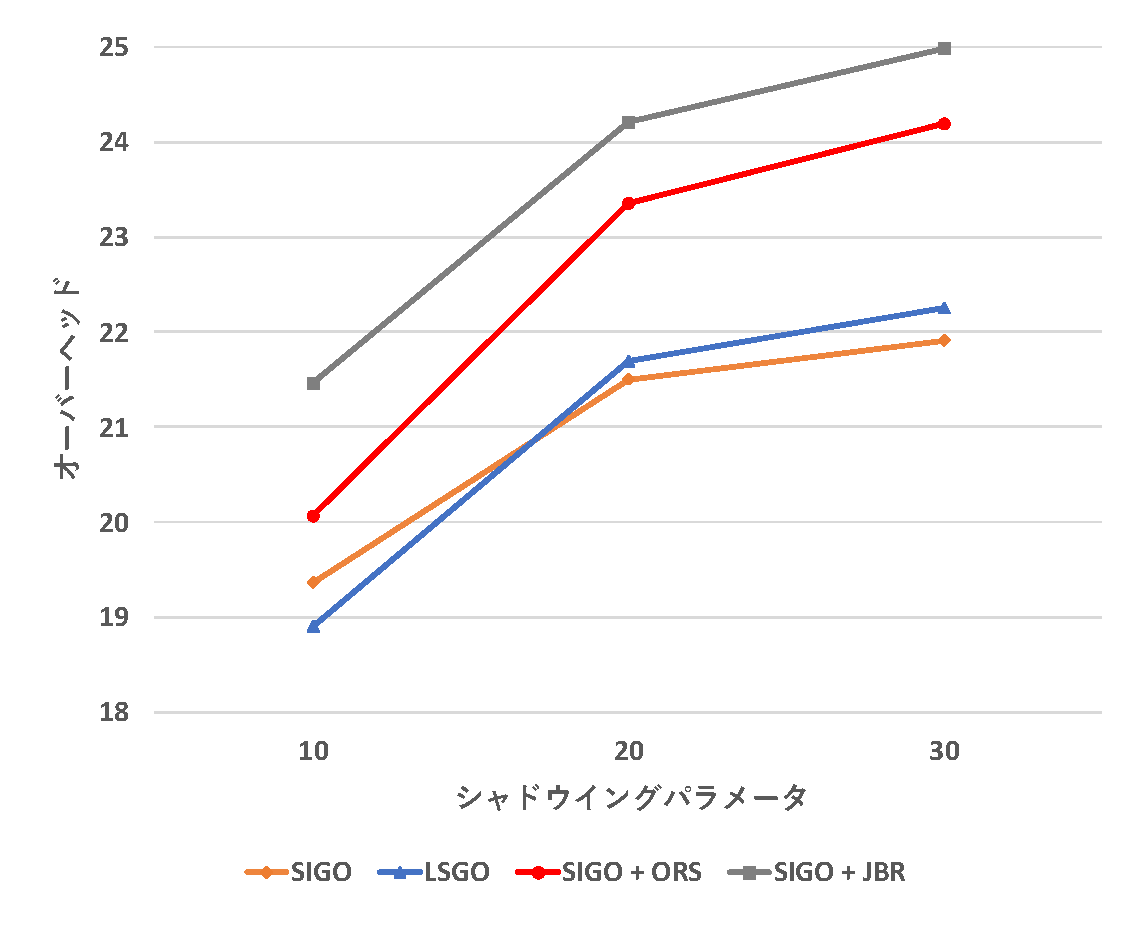
\includegraphics[width=120mm]{figures/SIGO_overhead_shadow.eps}
	\caption{オーバーヘッド vs シャドウイング強度}
	\label{fig:SIGO_overhead_shadow}
\end{figure}

\begin{figure}[!ht]
	\centering
	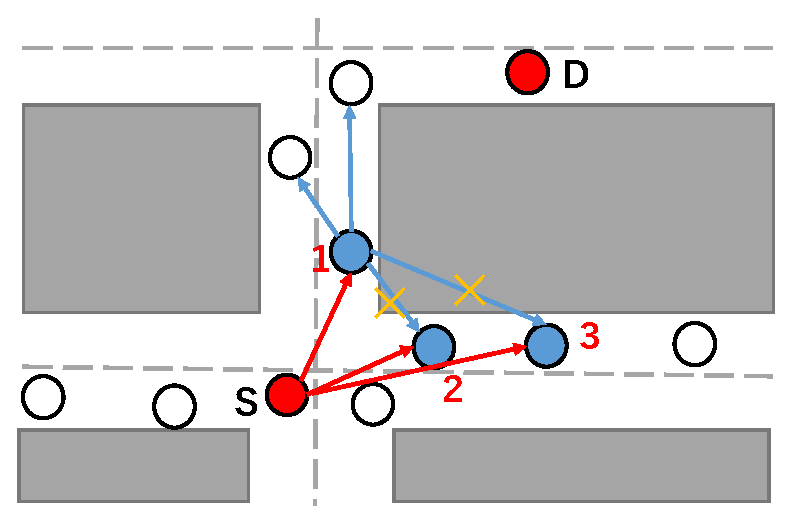
\includegraphics[width=100mm]{figures/dif_roadsegment_overhead_reason.eps}
	\caption{シャドウイング強度の増加によりオーバーヘッドが増加する原因}
	\label{fig:dif_roadsegment_overhead_reason}
\end{figure}




\section{Geocast routingの評価}
\label{Geocast_evaluation}


\subsection{評価項目}
\label{geocast_evaluation_item}
本シミュレーションでは, GSIGOの通信性能を評価するためパケット到達率(PDR), オーバーヘッド(Overhead)の2つの評価項目で評価した. またGSIGOと同様の手順でLSGOをGeocast routingに拡張したGLSGOと比較を行った. PDR, Overheadの算出式をそれぞれ式\ref{Geocast_PDR}, \ref{Geocast_overhead}に示す.

\begin{equation}
	\label{Geocast_PDR}
	PDR = \frac{GN_{recv}}{  GN  } \times 100
\end{equation}

ここで, PDRはソースノード(データパケットを一番初めに生成したノード)がデータパケットを送信したタイミングにGeocast Regionに存在するノードの中でデータパケットを正常に受信したノードの割合を表す. $GN_{recv}$はGeocast Regionに存在するノードでデータパケットを受信したノード数, $GN$はGeocast Regionに存在するノード数を表す. 

\begin{equation}
	\label{Geocast_overhead}
	Overhead =  \frac{  N_{sent}  }{GN_{recv}}
\end{equation}

ここで, オーバーヘッドはGeocast Regionに存在する1つのノードにデータパケットを届けるために必要なパケット数を表す.
$N_{Sent}$はデータパケットの総数を表す. 

\subsection{パケット到達率 : ノード数}
図\ref{fig:GSIGO_PDR_num}は, ノード数を変化させたときのPDRを示している.
図に示す通り, PDRの評価では以下の結果が得られた.
(1) ノード数が増加するほど, GSIGO, GLSGOともにPDRが増加する. 
(2) ノード数が増加するほど, GSIGOはGLSGOと比較してPDRが増加する.
(1) の結果は, ノード数が増加するほど送信ノードの隣接ノード数が増加し, 結果としてRCS数が増加するからだと推測できる.
(2) の結果は, ノード数が増加するほど送信の隣接ノードの中に, 交差点ノードが存在する確率が増加するため, GSIGOはGLSGOと比較して交差点ノードを中継候補ノードとして選択することでLocal optimum problemに陥る確率が減少したからだと推測できる.


\begin{figure}[!ht]
	\centering
	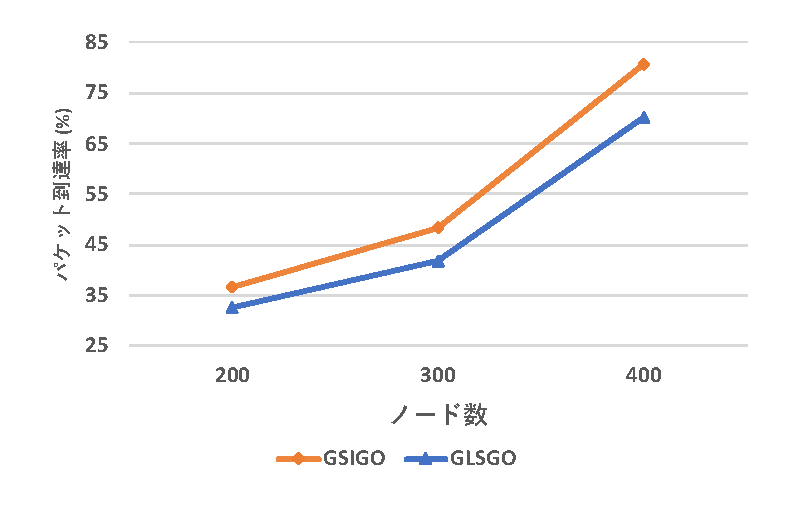
\includegraphics[width=110mm]{figures/GSIGO_PDR_num.eps}
	\caption{Geocast パケット到達率 vs ノード数}
	\label{fig:GSIGO_PDR_num}
\end{figure}

\subsection{オーバーヘッド : ノード数}

図\ref{fig:GSIGO_overhead_num}は, ノード数を変化させたときのオーバーヘッドを示している.
図に示す通り, オーバーヘッドの評価では以下の結果が得られた.
(1) ノード数が増加するほどGSIGO, GLSGOともにオーバーヘッドが減少する.
(2) ノード数に関係なくGSIGOとGLSGOの差は極めて小さい.
(1) の結果は, ノード数が増加するほど式\ref{Geocast_overhead}における$N_{Sent}$の数は増加するが, それ以上に$GN_{recv}$が増加したからだと推測できる.
(2) の結果は, GSIGOはGLSGOと比較してパケット数を増大させずに, パケット到達率が向上していることを示している. 

\begin{figure}[!ht]
	\centering
	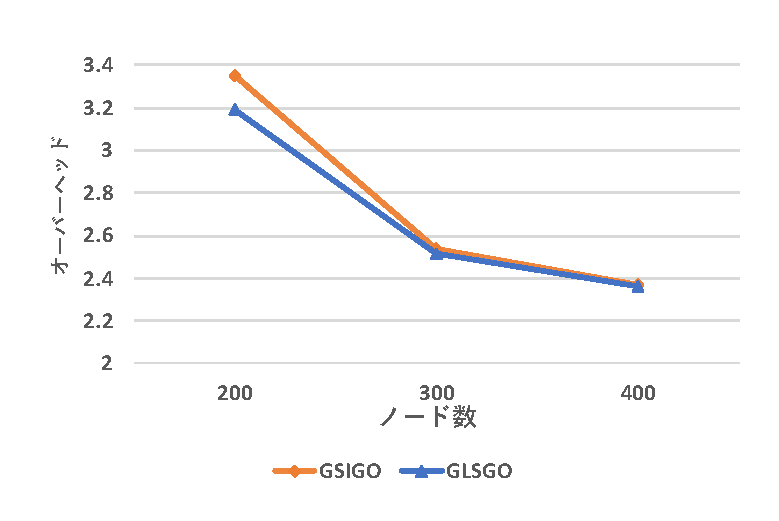
\includegraphics[width=110mm]{figures/GSIGO_overhead_num.eps}
	\caption{Geocast オーバーヘッド vs ノード数}
	\label{fig:GSIGO_overhead_num}
\end{figure}

\subsection{パケット到達率 : シャドウイング強度}

図\ref{fig:GSIGO_PDR_shadow}は, シャドウイング強度を変化させたときのPDRを示している.
図に示す通り, PDRの評価では以下の結果が得られた.
(1) シャドウイングパラメータが増加するほどGSIGO, GLSGOともにPDRが減少する.
(2) シャドウイングパラメータに関係なく, GSIGOはGLSGOと比較してPDRが増加する.
(1) の結果は, シャドウイングの影響でGeocast Regionに到達するデータパケット数が減少したことと, Geocast Regionに存在するノードによるデータパケットのブロードキャストパケットをシャドウイングの影響で受信できないノードが増加したからだと推測できる.
(2) の結果は, SIGOとLSGOとの比較ではシャドウイングパラメータが増加するほど差が大きくなったが, Geocast Routingにおいては, GSIGOはGLSGOと比較してシャドウイングパラメータが増加するほどGeocast Regionに到達するデータパケット数は増加したが, Geocast Region内でデータパケットが拡散される確率が減少したため, シャドウイングパラメータが増加してもGSIGOとGLSGOの差が増加しなかったと推測される. 

\begin{figure}[!ht]
	\centering
	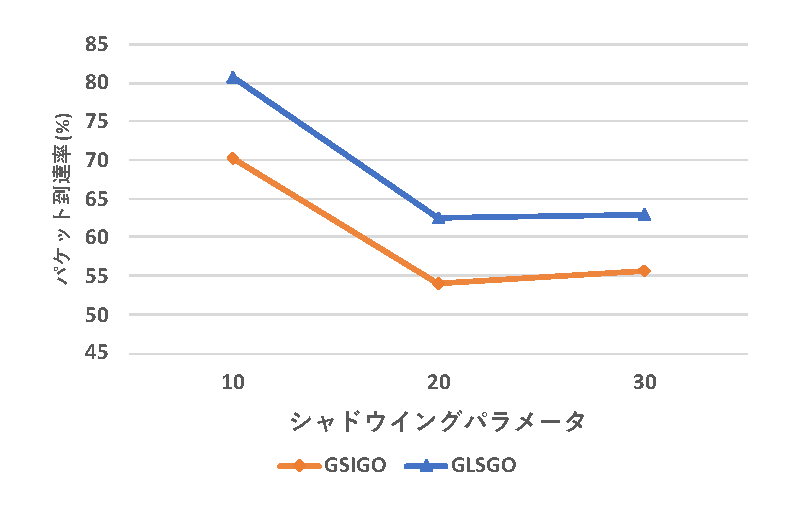
\includegraphics[width=110mm]{figures/GSIGO_PDR_shadow.eps}
	\caption{Geocast パケット到達率 vs シャドウイング強度}
	\label{fig:GSIGO_PDR_shadow}
\end{figure}


\subsection{オーバーヘッド : シャドウイング強度}

図\ref{fig:GSIGO_overhead_shadow}は, シャドウイング強度を変化させたときのオーバーヘッドを示している.
図に示す通り, シャドウイングパラメータに関係なく, GSIGOとGLSGOの差は小さかった. これはGSIGOがGLSGOと比較してパケット数を増大させずにパケット到達率を向上させていることを示している.

\begin{figure}[!ht]
	\centering
	\includegraphics[width=110mm]{figures/GSIGO_overhead_shadow.eps}
	\caption{Geocast オーバーヘッド vs シャドウイング強度}
	\label{fig:GSIGO_overhead_shadow}
\end{figure}




\chapter{結論}
\label{Conclusion}
本研究では, 既存Oppotunistic routingがシミュレーションでシャドウイングの影響を評価できていない問題, それが原因でルーチングプロトコルを設計するにあたってシャドウイングの影響を考慮できていないという問題に着目し, シャドウイング強度が増加するほどLocal optimum problemなどの問題が起こる可能性が高まり, 通信性能が低下することを示した. また, シャドウイングが引き起こす問題に対処するために, シャドウイングの影響を受けにくい経路を形成するSIGOを提案し, パケット到達率の向上とオーバーヘッドの削減を示した. また, Local optimum problemに対処する新たなRecovery StrategyであるORSを提案した. ORSは従来のRecovery Strategyと比較して, パケット到達率の向上とオーバーヘッドの削減を示した. さらにSIGOをGeocast routingに拡張したGSIGOを提案しGeocast routingにおいても有効な転送方式であることを示した. 今後の課題として, CRS数の最適化アルゴリズムの提案と様々な道路構造に対応するアルゴリズムの設計, 評価が必要である.


\addcontentsline{toc}{chapter}{謝辞}
\chapter*{謝辞}
\sloppy 

本論文では筆者が立命館大学大学院情報理工学研究科におい
て行なった「VANETにおける車両位置とリンク状態を考慮した地理的
opportunistic routing」」の成果をまとめたものである.

本研究を遂行するにあたり,全過程を通じて懇切丁寧なる御指導,御鞭撻を賜わっ
た,立命館大学情報理工学部野口~拓教授, 徳島大学大学院社会産業理工学研究部Alberto Gallegos Ramonet助教に深甚なる感謝の意を表す.

立命館大学情報理工学部において,御指導,御教授を賜わった立命館大学情報理工学部上山~憲明教授, 前田~忠彦教授, 西村~俊和准教授, 山本~寛教授,を始め,各教員の方々に衷心より御礼申し上げる.

ネットワークシステム研究室の諸兄には,日頃より多くの御助言,御協力戴き,種々の面でお世話になった.ここに深謝申し上げる.

ここに記して,以上の方々に深甚なる感謝の意を捧げる.

\addcontentsline{toc}{chapter}{参考文献}

%\newpage

\bibliographystyle{IEEEtran}
\bibliography{shuto}

\addcontentsline{toc}{chapter}{発表論文}
\chapter*{発表論文}

[1]高橋 柊人, 吉田 政望, ガジェゴス ラモネト アルベルト, 野口 拓, "VANETを用いた速度超過車両検出のためのブロードキャスト制御法", 2020年電子情報通信学会総合大会, 2020年3月

[2]高橋 柊人, 吉田 政望, ガジェゴス ラモネト アルベルト, 野口 拓, "交差点における建物遮蔽とリンク状態を考慮した地理的 opportunistic routing", 信学技報, vol.120, no.183, pp.48-53, 2020年10月

[3]Shuto Takahashi, Masami Yoshida, Alberto Gallegos Ramonet, Taku Noguchi, "Shadowing-Fading-based Intersection Geographic Opportunistic Routing Protocol for Urban VANETs", ICACT2020 24th International Conference on Advanced Communications Technology(2月発表予定)

\end{document}
